\documentclass[sigplan,anonymous]{acmart} %,review


%\usepackage[colorlinks=true,urlcolor=black]{hyperref}
\usepackage{booktabs}
\usepackage{url}
\usepackage{microtype}
\usepackage{tikz}
\usetikzlibrary{shapes.geometric, arrows}
\usepackage[xcolor=orange]{changes}
\definechangesauthor[name={Claudio Menghi},color=orange]{CM}
\usepackage[colorinlistoftodos,prependcaption,textsize=tiny]{todonotes}
\usepackage{xspace}
\usepackage{pifont}% http://ctan.org/pkg/pifont
\newcommand{\cmark}{\ding{51}}%
\newcommand{\xmark}{\ding{55}}%

\usepackage{graphicx} % for pdf, bitmapped graphics files
\usepackage{verbatim}
\usepackage[export]{adjustbox}
\usepackage{comment}
\usepackage{ifthen}
\usepackage{amssymb}
\usepackage{threeparttable}
\usepackage{tabu}
\usepackage{array}
\newboolean{showcomments}
\setboolean{showcomments}{true} % toggle to show or hide comments
\ifthenelse{\boolean{showcomments}}
  {\newcommand{\nb}[2]{
    \fcolorbox{gray}{yellow}{\bfseries\sffamily\scriptsize#1}
    {\sf\small$\blacktriangleright$\textit{#2}$\blacktriangleleft$}
   }
   \newcommand{\version}{\emph{\scriptsize$-$working$-$}}
  }
  {\newcommand{\nb}[2]{}
   \newcommand{\version}{}
  }
%\ifthenelse{\boolean{showcomments}}
%  {\newcommand{\ts}[4]{
%    \fcolorbox{black}{green}{\bfseries\sffamily\scriptsize#1 #2 - (Resp: \textit{#3})}
%    {\sf\small$\blacktriangleright$\textit{#4}$\blacktriangleleft$}
%   }
%  }
%   {\newcommand{\ts}[2]{}
%  }    
\newcommand\tb[1]{\nb{Thorsten}{#1}}
\newcommand\engineer[1]{\nb{Engineer}{#1}}
\newcommand\claudio[1]{\nb{Claudio}{#1}}
\newcommand\swaib[1]{\nb{Swaib}{#1}}
\newcommand\patrizio[1]{\nb{Patrizio}{#1}}

\newcommand\parhead[1]{\vspace{.26mm}\noindent\textbf{{#1}}}
\newcommand\parheadit[1]{\vspace{.26mm}\noindent\textit{{#1}}}
\newcommand{\secref}[1]{Sec.\,\ref{#1}}
\newcommand{\figref}[1]{Fig.\,\ref{#1}}
\newcommand{\Figref}[1]{Figure\,\ref{#1}}
\newcommand{\tabref}[1]{Table\,\ref{#1}}
\newcommand{\lstref}[1]{Listing\,\ref{#1}}


\newcommand{\picaxe}{PICAXE\xspace}
\newcommand{\easyc}{EasyC\xspace}
\newcommand{\edison}{Edison software\xspace}
\newcommand{\ardublockly}{Ardublockly\xspace}
\newcommand{\openroberta}{Open Roberta\xspace}
\newcommand{\arcbotics}{Arcbotics' SparkiDuino\xspace}
\newcommand{\missionlab}{MissionLab\xspace}
\newcommand{\flyaq}{FLYAQ\xspace}
\newcommand{\tivipe}{TiViPE\xspace}
\newcommand{\aseba}{Aseba\xspace}
\newcommand{\sphero}{Sphero\xspace}
\newcommand{\vex}{VEX Coding Studio\xspace}
\newcommand{\robotmesh}{Robot Mesh Studio\xspace}
\newcommand{\trik}{TRIK Studio\xspace}
\newcommand{\makeblock}{Makeblock 5\xspace}
\newcommand{\metabot}{Metabot\xspace}
\newcommand{\marty}{Marty software\xspace}
\newcommand{\tello}{Tello Edu App\xspace}
\newcommand{\codelab}{Code Lab\xspace}
\newcommand{\lego}{LEGO Mindstorms EV3\xspace}
\newcommand{\choregraphe}{Choregraphe\xspace}
\newcommand{\blocklyprop}{BlocklyPro\xspace}
\newcommand{\ozoblockly}{Ozoblockly\xspace}
\newcommand{\minibloq}{MiniBloq\xspace}
\newcommand{\turtlebot}{Turtlebot3-blockly\xspace}
\newcommand{\makecode}{Makecode\xspace}
\newcommand{\scratchev}{Scratch Ev3\xspace}
\newcommand{\enchanting}{Enchanting\xspace}
\newcommand{\robotc}{RobotC\xspace}

\usepackage[normalem]{ulem} % for \sout
\usepackage{xcolor}
\newcommand{\ra}{$\rightarrow$}
\newcommand{\ugh}[1]{\textcolor{red}{\uwave{#1}}} % please rephrase
\newcommand{\ins}[1]{\textcolor{blue}{\uline{#1}}} % please insert
\newcommand{\del}[1]{\textcolor{red}{\sout{#1}}} % please delete
\newcommand{\chg}[2]{\textcolor{red}{\sout{#1}}{\ra}\textcolor{blue}{\uline{#2}}} % please change

\copyrightyear{2019}
\acmYear{2019}
%\setcopyright{acmlicensed}
\acmConference[SLE'19]{12th International Conference on Software Language Engineering}{October 20--22, 2019}{Athens, Greece}
%\acmBooktitle{23rd International Systems and Software Product Line Conference - Volume A (SPLC '19), September 9--13, 2019, Paris, France}
\acmPrice{15.00}
%\acmDOI{10.1145/3336294.3336302}
%\acmISBN{978-1-4503-7138-4/19/09}


\begin{abstract}
Mobile robots are becoming increasingly important, fulfilling missions that support our everyday life. Hardcoding these missions is usually not feasible, given the uncertainty of the tasks the robots, or teams of robots, should execute.
Flexibility in programming such robots is necessary, which led to the proposal of many different languages enabling end-users to program robots. In fact, almost any commercial robot is equipped with a language-oriented environment that allows end-users to specify missions.

Our long-term goal is to build better languages, easing the specification of missions, ideally on a higher abstraction level. To this end, we need to improve our empirical understanding of the current state-of-the art of such languages and their environments. In this paper, we contribute in this direction. We present a survey of 29 mission specification environments for mobile robots that come with a visual and end-user-oriented language.
%A lot of work is being done in enabling end-users to flexibly specify robot missions. However it is not clear what features are offered in these environments.
We explore the design space of these languages and their environments, identify their concepts, and organize them as features in a feature model.
%We find that the majority of environments rely on projectional editing as opposed to parser-based editing, with imperative control flow paradigm, minimal interpretive semantics, and bare closeness of mapping to non-robotic and non-software engineering domains.
We believe that our results are valuable to practitioners and researchers designing the next generation of mission specification languages in the vibrant domain of mobile robots.

\end{abstract}
\begin{document}



\title{The Design Space of Visual Languages\\for Specifying Robotic Missions}
%\subtitle{for specifying Robotic Missions}
%A Survey of Mission Specification Environments for Mobile Robots

\renewcommand{\shorttitle}{Design Space of Visual Languages for Specifying Robotic Missions}

\maketitle


%%%%%%%%%%%%%%%%%%%%%%%%%%%%%%%%%%%%%%%%%%%%%%%%%%%%%%%%%%%%%%%%%%%%%%%%%%%%%%%%



%%%%%%%%%%%%%%%%%%%%%%%%%%%%%%%%%%%%%%%%%%%%%%%%%%%%%%%%%%%%%%%%%%%%%%%%%%%%%%%%
\section{Introduction}
Over the last decades, robot have become increasingly present in our everyday's life. Autonomous service robots that move around freely, following defined missions to accomplish replace humans in repetitive, laborious, or dangerous activities, often interacting with humans or other robots. The World Robotic Survey\footnote{https://ifr.org/ifr-press-releases/news/world-robotics-survey-service-robots-are-conquering-the-world-}\tb{guys, please do not put a URL tag around! will prevent line break} estimates a whopping 35 million indoor service robots to be sold by 2018, accumulating a sales value of \$12 billion since 2015. The global sales of household and personal robots is expected to grow by 23.5\,\% per year\,\cite{sheng:online}, accompanied with progresses in robot technology, especially in image processing, planning, control, and collaboration.

Robotic systems, such as service, industrial, military, or space robots, are among the most complex autonomous systems today. Different techniques have been proposed for engineering the various aspects of robotic behavior\,\cite{Fernandez-Perdomo2010,DiRuscio2014,Doherty2013,AtrickD..Ulam2010}. For instance, \citet{Kolling2016} identify core concepts needed to design a human-swarm interaction. A meta evaluation of human-system-interfaces controlling semi-autonomous swarms was conducted by \citet{Hocraffer2017}, who identified advantages, challenges, and limitations of interfaces for Unmanned Aerial Vehicles (UAV). \citet{Mohamed2008} analyze middleware used in robotic engineering to achieve interoperability of components. A taxonomy of multirobot target detection and tracking is provided by \citet{Robin2016}.

\looseness=-1
Engineering robotics control software is challenging. Specifying the behavior of a robot---typically called the robot's mission---has been among the most complex tasks of a robotics software engineer. Developing missions has long required substantial expertise\,\cite{Brugali2009,Aragao2016}, for instance, using logical languages such as LTL or CTL or other intricate formalisms to specify missions\,\cite{Luckcuck2018}.
However, over the last two decades, a range of more end-user-oriented programming environments appeared; They allow the specification of the mission of robots in a more user-friendly way, and this alleviates the need for intricate programming skills not readily available for end-users\,\cite{Weintrop2018,Bozhinoski2016b}. On the other hand, it is exactly those end-users who know the details about the missions to achieve.

%The end-users best know what they want the Robots to do for them, but not how to program robots.  Robots could be multi-purpose and developers cannot anticipate all the possible use of the robots. 
%On the other hand robot engineers and robot software developers understand how the Robot works but are not always familiar with what the End-user expects from the robot system. 

%This calls for End-user programming\,\cite{Weintrop2018}, where users can express in concrete syntax what they expect the robot to do for them.

Researchers and practitioners have invested substantial effort into achieving end-user-oriented programming of robots\,\cite{Weintrop2018,Biggs2003,Bozhinoski2016b,Arts2010,Nordmann2016a}. In fact, almost every commercial mobile robot nowadays is distributed with an environment for programming the behavior, called \emph{mission-specification environment} in the remainder. Such environments rely on dedicated Domain Specific Languages (DSLs) that end-users can utilize to specify missions.
 %robot programming, using related synonyms like; robot behavior programming, task programming, mission specification, robot visual programming, graphical robot programming as asserted in literature
One of the first surveys of DSLs in robotics is provided by Nordmann et al.\,\cite{Nordmann2014,Nordmann2016a}; yet, none of the DSLs covers mission specification. While surveys on mission-specification techniques and environments exist\,\cite{Biggs2003,Bravo2018,Luckcuck2018},
none of them covers the area of mission specification environments to understand the key features and how they enhance mission specification. However, most of these language still appear to be relatively low-level and limited to simple behavior specifications.

To build the next generation of mission-specification languages and environments, we need to improve our empirical understanding of the current state-of-the-art in mission specification. Our focus is on end-user-oriented languages providing a visual syntax. In our study, we identify open-source and commercial environments that allow end-user-oriented mission specification of robots. While robot programming environments consider all programmable aspects of the robot system, this study focused on environments in which robot missions are created, designed or particularized. Specifically, we consider a mission specification environment as a collection of tools that facilitate definition and stipulation of robot tasks that form a mission. We study the environments' and their languages' main characteristics and capabilities---which we model as features in a feature model\,\cite{kang.ea:1990:foda,damir2019principles}---a common research method. %---pertaining to mission specification. 

%We achieved this by collecting specification environments that exist in the user domains, with their characteristic features and establish how they differ from one another based on the research questions below. 29 environments were selected for the study, language and programming features were extracted and modeled the environments into a feature model to better understand what the languages offer to support end-user programming of robot(s).

%The main goal of the study is to provide language designers with a feature model as an instrument that helps in designing the most suitable language and its associated environment depending on needs at hand. To solve this problem we extract key features that differentiate mission specification environments; with the view of understanding the language features and mission specification concepts implemented in these environments.

We formulated two main research questions:

\textbf{RQ1}: \textit{What visual, end-user-oriented mission specification environments have been presented for mobile robots?}
We systematically and extensively identify such environments from various sources, including the Google search engine and literature search using snowballing techniques. Among others, this includes open-source, but also commercial environments for which substantial material (e.g., documentation or scientific papers) to analyze them exists.

\textbf{RQ2}: \textit{What is the design space in terms of common and variable characteristics (features) that distinguish the environments?} Our focus is on understanding the concepts that these environments and their languages offer that end-users utilize to specify the missions of mobile robots. We conduct a feature-based analysis, resulting in a feature model detailing our results in terms of features organized in a hierarchy.

%\textbf{RQ3}: How mission specification environments differ?\\
%By consideration features in the respective environments we seek to identify how environment differs among each other. 
%This will  help users understanding the most suitable mission specification environment depending on their needs.\\ 
%\claudio{Notation. choose among end-user and end-user and mission specification and mission specification and be consistent}

We identified a total of 29 environments, whose environment capabilities, general language characteristics, and, most importantly, language concepts we study and organize in a feature model to understand the overall design space of existing environments.
%language and programming features were extracted and modeled the environments into a feature model to better understand what the languages offer to support end-user programming of robot(s).
We believe that our work is valuable to practitioners, researchers, and tool builders developing the next generation of mission-specification languages and environments. The feature model shows the mandatory features that all environments have, as well as many optional features only some realized---inspiring future language design.

%The motivation of this study is to provide language designers with empirical understanding of the start-of-the-art in robot mission specification languages in form of a feature model by exploring the language design space and their environments.    


%\claudio{Provide a designer with an instrument (the FM) that helps in selecting the most suitable environment depending on her needs).} 

\section{Background}
A typical robot mission is specified by a user by programming a behavior, which the robot exhibits during execution. The mission specified is either compiled into robot executable sequence of instruction or directly interpreted depending on the semantic support. During deployment the executable file is transferred to the robot either by cable connection or wireless. Environments that support live programming enable users to specify such missions at run-time. Visual languages are often based on established third-party libraries such as Blockly \cite{blockly} and Scratch \cite{Kaucic2015}. These are typically customized to incorporate domain-specific blocks as new language concepts---representing robotic and end-user domain mission primitives, such as move forward/backwards, read sensor, and turn right/left.

%\tb{can you briefly describe the process of mission specification here and how environments look like; for instance, explain the typical libraries, Blockly and Scratch (see below) that are used to realize domain-specific languages}

$\bullet$ \emph{End-user facing:} an environment that is target for being used by non expert end-users. %\deleted[id=CM]{The environment provides concrete syntax to end-users for specifying tasks.}\\

$\bullet$ \emph{Specification of Robotic mission:} the definition of the goal of the robotic application or the tasks that must be performed by the robot(s).

$\bullet$ \emph{Specification  Environment:} a collection of language tools and features with abstraction support for robotics and end-users, suitable for the definition and execution of robotic missions.

$\bullet$ \emph{Mobile Robots:} robots with ability to change  their locations in space like: drones, mobile manipulators, mobile platforms, mobile humanoids, vacuum cleaner robots.

$\bullet$ \emph{Declarative vs imperative mission:} a declarative mission allows end-users to specify what to be achieved i.e., a mission goal without saying how the goal is achieved. While an  imperative mission allows end-users to specify the precise actions and movements to be accomplished in order to satisfy the mission goal. % set of tasks in their order of execution. %Imperative  mission specification  are usually specified by user domain experts who exactly know how the mission tasks are executed.\\

$\bullet$ \emph{Block:} a graphical symbol or icon  which represents  a language construct; for example ``moves steering" block in LEGO, ``if do else" block in Open Roberta ~\cite{OpenRoberta}. Blocks are used to build a mission. %\\ %\claudio{Remove (comment)}

$\bullet$ \emph{Blockly:} is a library proposed by Google\,\cite{blockly}, which provides support for creating graphical notations, where each block represents a programming concept. %The library is used for building web based and mobile applications with graphical notations.\\ https://developers.google.com/blockly/guides/overview %\claudio{Remove Blockly (comment)}
%Common examples we captured in this study include Google
%Blockly blocks enforce semantic correctness of the program by allowing two blocks to connect only if they make semantic sense\tb{no, that's not what Blockly can do, that's the responsibility of the semantics realization of the actual DSL of each environment}.
%Code can be generated as; python, JavaScript or PHP.
The library can be extended to define new blocks, support functions, and procedures. Blockly allows access to the parse tree, and is flexible to generate code in target language\,\cite{Passault2016}. Scratch is a variant of Blockly created by the Massachusetts Institute of Technology media laboratory. It can be used to create stories, games, animations, music and art projects~\cite{Kaucic2015}. The library can be extended by adding custom blocks to suit needs of the end-user domain. %\tb{also explain scratch as a library, similar to blockly}

%\parhead{Educational Robotics}
%Mobile robots have been recognized as an ideal vehicle to teach basic programming skills to children and students. As such, a large variety of educational robots has been proposed, such as Lego Mindstorms, Softbank Robotics' NAO or Pepper\tb{to be continued}
%As we will show, the majority of our environments supports educational robots}

\section{Methodology}
We now describe how we selected our subjects (\secref{sec:sel}) and how we classified their features (\secref{sec:extr}).
 
\subsection{Identification of Subject Environments (RQ1)}
\label{sec:sel}
\looseness=-1
We are interested in environments that support end-user programming of mobile robots. Such environments should provide domain-specific languages for specifying robotic missions (i.e., behaviors and tasks). %Our focus was on environments targeting novice programmers with graphical notations, which we systematically
%We identified the environments from the following data sources  using inclusion and exclusion criteria. 
\Figref{fig:selection} illustrates how the environments were identified from the following data sources.

%---including languages that are close to the robotics domain---
\looseness=-1
\parhead{Data Sources.}
We used three different data sources: (i) input provided by the authors based on experience and knowledge in the field, (ii) the Google search engine, and (iii) forward and backward snowballing upon a set of related survey papers.
%These candidates were then filtered based on explicitly formulated inclusion and exclusion criteria (explained shortly).

%Since a web search for ``robot mission'' alone would not return enough relevant results, we designed a systematic search taking into account multiple sources, varying terminologies (programmable robots, robot programming environment or mission specification environment).  and explicitly defined inclusion and exclusion criteria.
%Specifically, our identification process involved data collection to identify environment candidates, then applying inclusion-exclusion criteria to the candidates, and finally identifying alternative environments\tb{not clear to me what the last point means}. 

\parhead{Identification of Candidate Environments.}
As a first step, we identified candidate environments---i.e., software for programming robots mentioned in a source that appeared to fit our study scope, but before applying dedicated inclusion and exclusion criteria (explained shortly)---using the following strategy.

\emph{(a) Environment candidates from experience.} From our past experience in robotics software engineering, we assembled a list of 25 candidate environments.

\emph{(b) List of mobile robots.} We created a list of 59 commercial mobile robots based on our past experience (e.g., we were aware of many educational robots, such as Thymio, Sphero or NAO) and from conducting a Google search (``mobile robot'').
%were aware of various robot programming environments, which led to 25 environment candidates. 
%The authors also created a list of 59 mobile robots based on experience, each person listing any mobile robots that he knows. \patrizio{then we contribute with our experience two different lists, one of non-commercial environments in the first item, and one of commercial environments in this item. At the beginning of the section we only mention one list. This should be clarified: it's confusing.}
From the robots' web pages, we identified that software that was offered for programming the robot missions, which gave us exactly 59 environment candidates.
%The respective robot websites and Google search using the robot name as search string  were used to identify the environments in which missions are specified for the robots.

\emph{(c) Google search.} We conducted a search with the search string \emph{("programmable robots" OR ("robot programming" OR "mission specification") environment) "mobile robot"}, which yielded 373 results (note that Google reported 774,000 results, which collapsed into 373 when selecting the last page).

\emph{(d) Snowballing.} Based on a list of six survey papers\,\cite{Biggs2003,Bravo2018,Jost2015,Luckcuck2018,Nordmann2016a,Hentout2017} we were aware of from our experience, we conducted snowballing. Specifically, we identified environment candidates from reading these survey papers and then from reading all papers being cited in each (backwards snowballing) and all papers citing it (forward snowballing), also ignoring duplicates. We identified 12 from \citet{Biggs2003}, 44 from \citet{Bravo2018}, 14 from \citet{Jost2015}, 0 from \citet{Luckcuck2018}, 6 from \citet{Nordmann2016a}, and 7 from \citet{Hentout2017}, totaling 83 candidates.
%Snowballing.
%1.	Six papers were identified
%2.	From each paper, environments were extracted. 
%3.	Forward snowballing: papers which reference the candidate papers were read to extract further environments.
%4.	Backward snowballing: papers in the reference list of the candidate papers were read to extract environments
%•	The environments extracted were then subjected to inclusion and exclusion criteria to generate the final list.
%•	Duplicate environments were removed.

%\claudio{Old}
%\begin{itemize}
 %   \item From our past experience in robotics software engineering, we were aware of various robot programming environments, which led to 25 environment candidates
    %\tb{really so many? I cannot remember that we came up with so many; where's the list?} \swaib{check "validation sheet" in the data collection spreadsheet}\tb{not sure where exactly, but I see sth. with 13. Please give the list to the co-authors in the chat for verification, also put as comments in this Latex file}.
%   \item The authors created a list of 59 mobile robots based on experience, each person listing any mobile robots that he knows. \patrizio{then we contribute with our experience two different lists, one of non-commercial environments in the first item, and one of commercial environments in this item. At the beginning of the section we only mention one list. This should be clarified: it's confusing.}\tb{afair, the list of mobile robots came from experience and a Google search} \tb{still need details}. 
 %   The respective robot websites and Google search using the robot name as search string  were used to identify the environments in which missions are specified for the robots. % \tb{?}\tb{how? I thought you checked the websites; if so, please write}\tb{how many?}.
   %\tb{reference then}
   %\tb{need details}
  %  \item We conducted a Google search with the search string \emph{("programmable robots" OR ("robot programming" OR "mission specification") environment) "mobile robot"}, which yielded 774000 results. However, after scanning through all the web pages returned,
%     \claudio{Did we really do that? 
%     Some calculation: by assuming we spent 10 minutes each it lead to 10750 days... good job! We should be a bit care full.
%     }
%     we found only 373 hits, a common phenomenon with Google search. 
%     \item For snowballing, six survey and review papers were identified on environments and languages.
%     %to \ugh{contact snowball}. \patrizio{if we identified 25 environment candidates in the previous step, why we identified only 6 papers? I would expect at least one paper for each candidate environment.} \swaib{The 6 papers are not specific to one environment and the 25 environments have not gone through inclusion and exclusion criteria}
%     %\ugh{Both forward snowball based on new papers which cite the candidate paper and backward snowball based on papers in the reference list of the candidate paper, were done}.
%     %\patrizio{write in active way, for instance: We performed both forward...} 
%     We performed both forward snowballing based on new papers which cite the candidate papers and backward snowballing based on papers in the reference list of the candidate papers. A total of 83 environments were identified \cite{Biggs2003} 12, \cite{Bravo2018} (44), \cite{Jost2015} (14), \cite{Luckcuck2018} (0), \cite{Nordmann2016a} (6) and \cite{Hentout2017} (7), totalling to 83 candidate environments.\tb{still need more details, incl. how many transitive relations you followed (not sure how this is called exactly in the snowballing literature, but there must be a measure of the number of levels etc.)}
%     \item We lastly used the robots programmed using the environments identified from the above data sources to identify alternative environments for programming them. This was done by doing Google search, with robot name as the search string as shown in \figref{selection}. \claudio{This goes in Section 3.2}
% \end{itemize}  

% \tb{did pass until here in this section}
In summary, we collected 537 candidate environments.

\parhead{Application of Inclusion and Exclusion Criteria.}
In the second step, we filtered the 537 candidates according to the following inclusion and exclusion criteria.

\noindent
 \emph{Inclusion Criteria.} We included a candidate when it fulfilled all of the following conditions. It must:
%\patrizio{be more clear. To be included any of the following should be true, some of them, only one?}
\begin{itemize}
\item allow the specification of missions for mobile robots; 
\item offer a domain-specific language with a visual notation targeting end users; % or a textual notation,
%\item is end-user-facing enabling user domain experts to specify a mission in the environment, 
\item come with documentation about the environment and its language;
\item be available to users in the sense that it is either sold or can be downloaded freely, in other words, has indications of being used by practitioners.
%in table \ref{tablelist} some environments were studied using documentation only. May be we have to remove them or remove the (I,W,D) column in the table. these include \flyaq, \tivipe, \missionlab, \aseba, \codelab, and \choregraphe }
\end{itemize}

\noindent
 \emph{Exclusion Criteria.} 
 An environment is excluded if any of the following conditions holds. It must not either:
\begin{itemize}
\item be an environment that focuses on programming system aspects of a robot, such as the Robotics Operating System (ROS), instead of specifying missions;
%are general purpose, \patrizio{what does it mean general purpose here?}
\item target non-mobile robots, such as stationary industrial robots, 3D printers or Arduino boards; 
%\patrizio{what about movable industrial robots? Should we be more precise, like non-movable industrial robots?}
%\item environments without mission specification aspects, which rather focus on robot architectures~\cite{Nordmann2016},\patrizio{how this differs from the first item - development environments that are not developed to specify robotic missions, but are general purpose ?}
\item be a mission control application with pre-programmed missions;
\item be a remote-control application for mobile robots.
%\patrizio{write better}
%\item the environment's documentation is only a loose collection of web pages, \patrizio{unclear}
%\item the environment should not be only remote control application (e.g., Drone control apps).\patrizio{primarily is ambiguous. How to measure if something is primarily or not? Explain better}
\end{itemize}

In summary, we selected 26 environments using the inclusion/ exclusion criteria from the initial collection of 537.

\parhead{Find Further Alternative Environments.} In a third step, we used the robots programmed using the environments identified from the above data sources to identify alternative environments for programming them. This was done through a Google search with the robot name as the search string.
In summary, we identified 40 robots from the 26 environments selected, which yielded three more environments. As such, our final number of environments identified is 29. \tabref{tab:DataSources} summarizes our results.

\begin{table*}[t]
\caption{Identified environments per step and data source (cf. \secref{sec:sel})}
\label{tab:DataSources}
\vspace{-.4cm}
\begin{smaller}
\begin{threeparttable}
\begin{tabular}{p{7cm}p{10cm}}\\
\toprule
\textsf{data source} & \textsf{identified environments}\\
\midrule
Environments from experience (25 candidates) & \missionlab, \choregraphe, \lego, \sphero, \tivipe, \aseba, \robotmesh, \edison, \makeblock, \trik, \ardublockly, \minibloq, and \flyaq. \\
List of mobile robots (59 candidates) & \picaxe, \openroberta, \arcbotics, \vex, \metabot, \marty, \tello, and \codelab. \\
Google search (373 candidates) & \missionlab, \choregraphe, \lego, \sphero, \tivipe, \aseba, \robotmesh, \edison, \makeblock, \trik, \ardublockly, \minibloq, \flyaq, \picaxe, \openroberta, \arcbotics, \vex, \metabot, \marty, \tello, \codelab,  \blocklyprop, and \ozoblockly.  \\  % -> what did "\codelab. unique" mean?
Snowballing (80 candidates) &  \lego, \missionlab, \aseba, \vex, \choregraphe, \minibloq,  \ozoblockly, \sphero, \tivipe, \openroberta, \trik, \robotmesh, \enchanting, \easyc and \robotc\\ % -> what did "\robotmesh unique" mean?
Further alternative environments\tnote{1}& \turtlebot, \makeblock, \scratchev \\
\bottomrule
\end{tabular}
\begin{tablenotes}
\item[1] Found by seeking alternative environments for robots supported by the identified environments above
\end{tablenotes}
\end{threeparttable} 
\end{smaller}
\end{table*}
%13 from the team:\missionlab, \choregraphe, \lego, \sphero, \tivipe, \aseba, \robotmesh, \edison, \makeblock, \trik, \ardublockly, \minibloq and \flyaq.  8 environments from mobile robot list: \picaxe, \openroberta, \arcbotics, \vex, \metabot, \marty, \tello, and \codelab.   Interestingly all the 21 from stage 1 and stage 2 were included in stage 3 plus 2 more: \blocklyprop, and \ozoblockly.  Stage 4 generated 15 environments, out of which 12 already exist in stage 3: the exclusive 3 are: \enchanting, \easyc and \robotc.  From alternative environments for robots, 3 selected are: \turtlebot, \makecode, and \scratchev. 

    \begin{figure}[t]
      \centering
      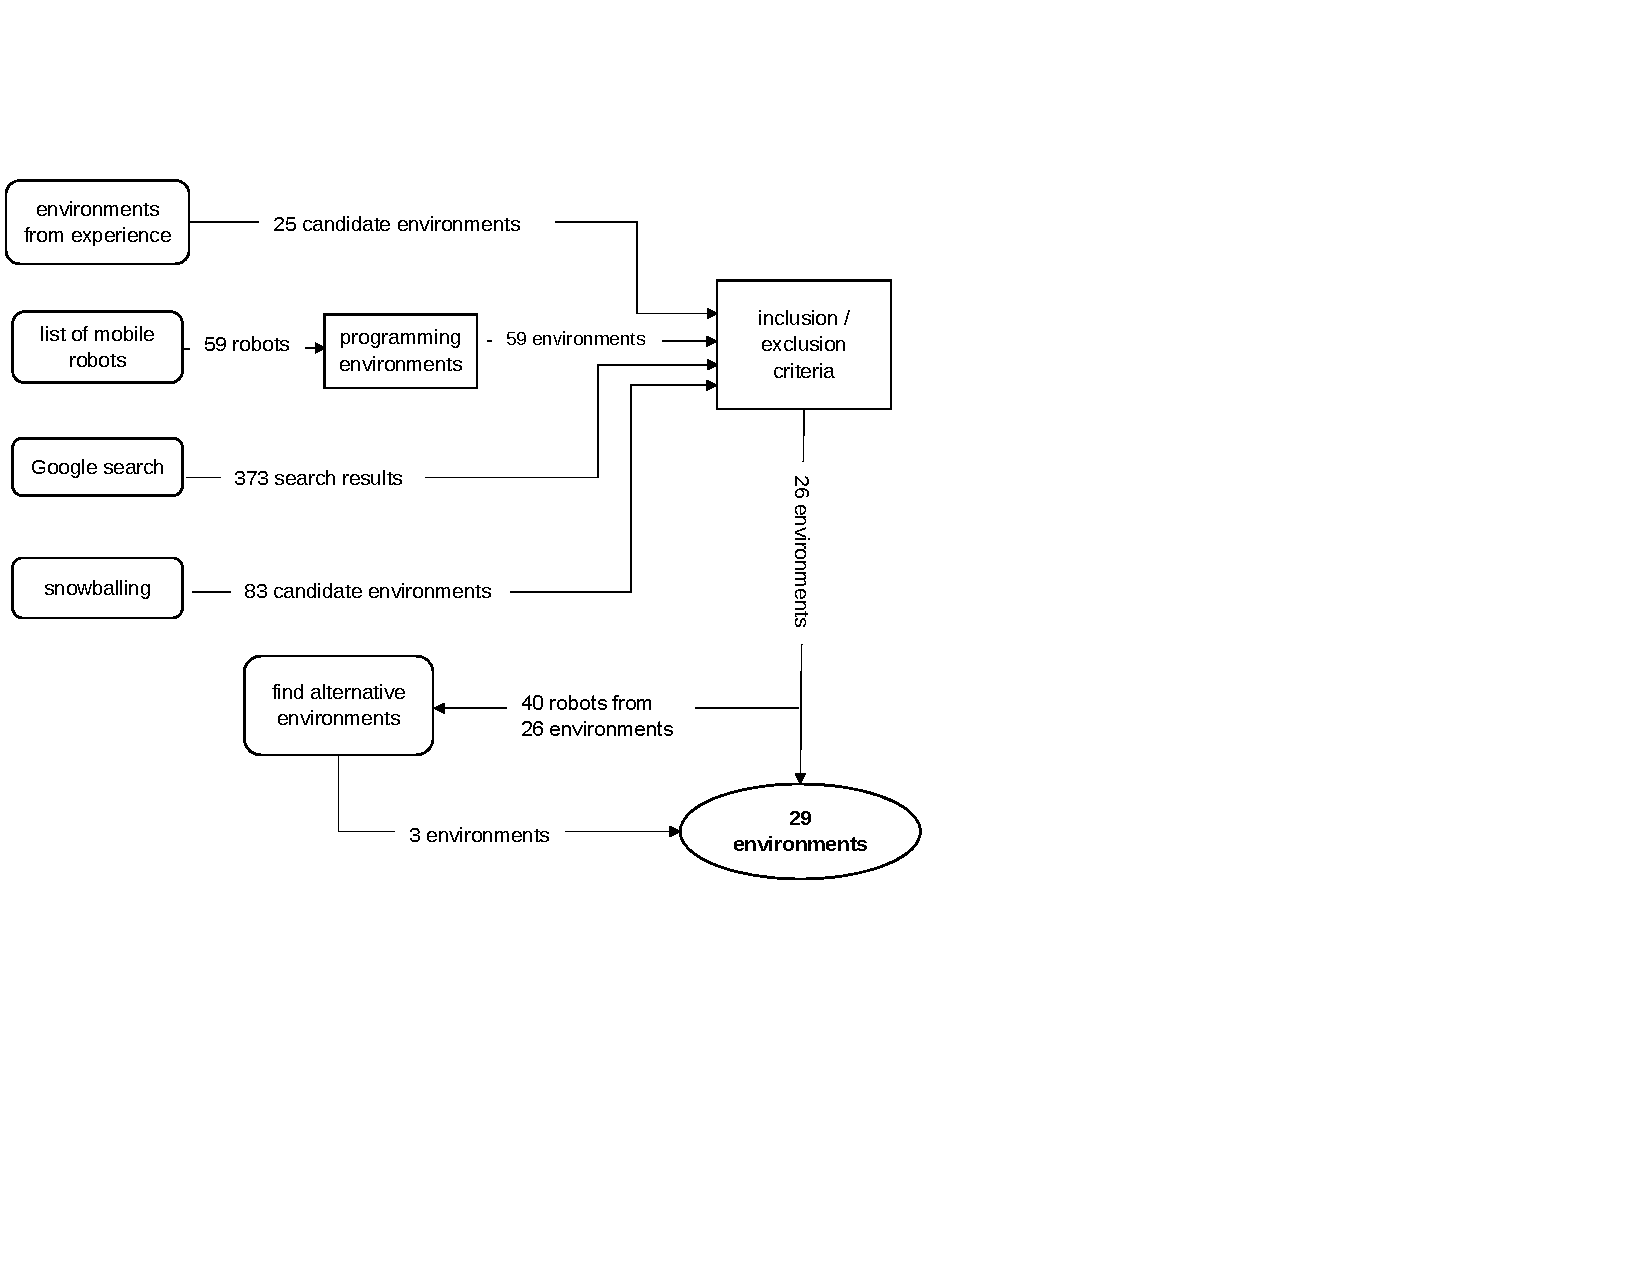
\includegraphics[width=\columnwidth]{fig/selection.pdf}
      %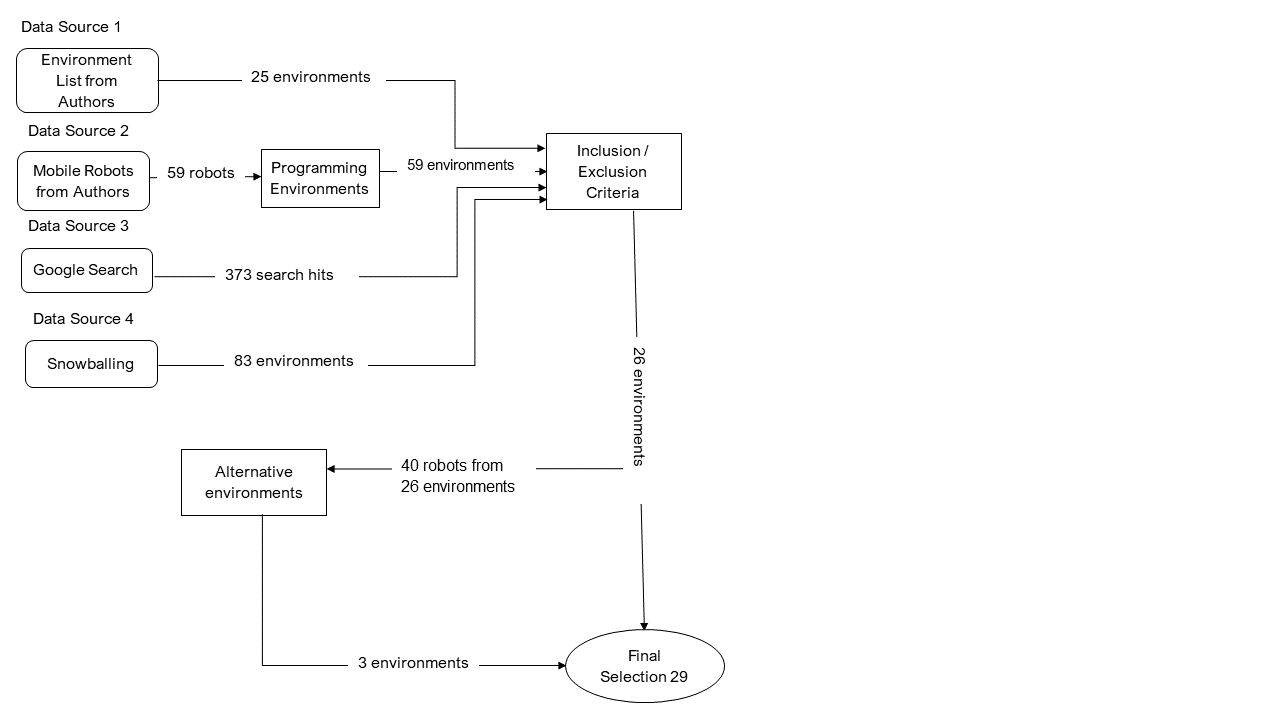
\includegraphics[width=\linewidth]{selection10.png}
      \caption{Identification of subject environments}
      \label{fig:selection}
			\vspace{-.4cm}
    \end{figure}
    

\subsection{Analysis of Identified Environments (RQ2)}
\label{sec:extr}
Our goal was to identify the characteristics that distinguish our subjects in the form of features\,\cite{berger2015feature} and to organize them in a feature model\,\cite{kang.ea:1990:foda,damir2019principles}. Performing such a feature-based analysis is a common method for comparing the design space of technologies, such as model transformations\,\cite{transformationSurvey}, language workbenches\,\cite{erdweg2013languageworkbenches} or variation control systems\,\cite{linsbauer2017gpce}.

The data sources for analyzing the identified environments were scientific papers about them, their websites, related documentation (e.g., user manuals or programming guides), and examples of missions expressed in the respective language.

 %Features were extracted from papers published on selected environments, environment websites, related documentations and  specification of sample missions. We used indirect data collection where researcher did not interact with the participants in this case the environment developers. The data collection technique was independent since the author only accessed the artifacts like publications, specification environments and related websites to extract data for the study\,\cite{Lethbridge2008}. The following steps were followed to extract features from the selected subjects:
%\begin{enumerate}

Our strategy was as follows.
First, in a brainstorming meeting, after an initial screening of the subjects, we identified key features of the environments---mainly representing the top-level and intermediate features in the feature model. Second, we consulted the websites to further identify key features and organize them in a hierarchy. This first skeleton provided the basis for an iterative refinement of the feature model by systematically, for each environment: (i) reading the scientific publications and other technical documentations about the environment; (ii) when possible, downloading and installing the environment to specify example missions, or alternatively for web-based environments, using the online tooling; and (iii) reading through the help menu for better understanding of how the environments are used to specify missions.

\looseness=-1
In this process, we iteratively refined the feature model and maintained a spreadsheet that contained notes about the realization of the individual features in each environment. The features were discussed among all authors to reach consensus.

%which were then confirmed and refined by an observational study of the selected environments. The brainstorming question used was: ``what mission specification features can be observed in mission specification environments?". 

%(b) General features were extracted from the respective environment websites. 
%
%(c) Read publications and other technical documentations about the environment. 
%
%(d) Downloaded and installed the environments to specify sample missions. Examples for web-based environments were run online.  
%
%(e) Read through the help menu for better understanding of how the environments are used to specify missions.
%The data was collected in a spreadsheet, then analyzed to construct the feature model. 
%%\claudio{Something about how features are connected} \swaib{some hint on how features are connected!}

%\subsection{How research questions were answered}
%\label{sec:answ}
%\noindent
%To answer RQ1, we collected data from multiple sources; teams suggested environments they knew, using mobile robot list we searched for their respective environments in which they are programmed. Snowballing was also done to identify environments mentioned in literature and Google search was also done to identified environments. Using the inclusion \& exclusion criteria we selected 29 environments, which we considered as end-user facing mission specification environments for the study.  RQ2 was answered by identifying features from: literature on selected environments, technical documentation and running sample missions in the environments. The resulting features were tabulated in a spreadsheet. 

\section{Mission Specification Environments}\label{sec:environments}

\tabref{tablelist} lists all identified environments in their studied version, detailing the supported operating system or environment (e.g., web), 

Some environments were installed (I), others are web based (W) while in other we relied on documentation (D) either as a website, technical documentation or publications about the environments. For environments which are not web based and were not installed, compatibility of software and software policy were  the main reasons for not installing them. Below are the environments selected for this study:

%\tb{Swaib, can you write a summary about the environments? (not much more than half a page); the original text is commented out below in the Latex file}
%\tb{is there a difference between block-based and blockly-based?} \swaib{blockly-based is an instance of block-based. Block-based means use of graph blocks/icons to represent programming concepts}


\begin{figure}[t]
     \centering
    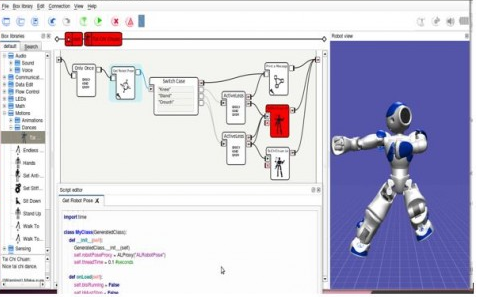
\includegraphics[width=\columnwidth]{choregraphe.png}
      \caption{The environment \choregraphe for the NAO robot}
      \label{fig:choregraphe}
   \end{figure}


%\begin{comment}
\parhead{\picaxe} (specifically, Blockly for Picaxe) is a programming environment for PICAXE chip-based robots such as the PICAXE 20X2 microbot. We study the \picaxe editor (PE), which provides textual (in a Basic-style language) and Flowchart-based programming, as well as the tool Blockly for \picaxe, relying on the Blockly library realizing the visual syntax.

%The current version PE6 provides graphical programming using either Blockly or Flow chart while text programming is done using Basic with simulation support~\cite{PICAXE}.% The environment has code generation wizards like pwmout and tune to generate code from the graphical notations.
%Logicator Flowcharting software is one of the programming techniques used in \picaxe in which flowcharting cells are used build a robot program. Such cells include: start, stop, process, and input.
%http://www.picaxe.com/Teaching/Logicator-Flowcharting-Software


\parhead{\ardublockly} is a Blockly-based graphical environment that generates python code for Arduino boards. The environment is used for programming Spartan robot ~\cite{Spartan}.% and can run on windows, Mac OS X, and Linux operating systems. The editor supports programming based on dragging and dropping of blocks, with code block warning and the code is compatible with variety of Arduino board based . 

\parhead{\openroberta} is a web-based environment for programming a variety of robots. It can either be run on the cloude or installed on a local server. The range of robots that can be programmed in Open Roberta include: Lego Mindstorms EV3, NXT, Calliope mini, micro:bit, Bot' n Roll[beta], Nao [beta], BOB3 [beta] ~\cite{OpenRoberta,Jost2015,Ketterl2015}. %The environment supports code generation in python, java, javascript and C/C++ depending on the particular robot being programmed. The graphical interface implements blockly code blocks for programming the robots. 

\parhead{\arcbotics} provides block-based programming environment for Sparki robot. The blockly based programs generate C/C++ code for the robot to execute~\cite{ArcboticSparki}. %The colourful blocks help in syntactic support during programming to guide right order of assembling the blocks. 

\parhead{\edison} is an environment that provides Edblocks and Edscratch graphical notation while Edpy for textual notation. The current versions of Edison robots supported are V1 and V2 ~\cite{Edison}.%As Edblock provides programming blocks in which programmer provides parameters of a block, Edscratch provides symbolic block which depicts what the block actually does. This makes Edscratch more closer to the user domain. The graphical notations generate code in python 

\parhead{\missionlab} provides a robot programming environment in which events and actions are specified in a state machine with graphical notation for multirobot missions. The missions can be executed on real robots; ATRV-Jr, Urban Robot, AmigoBot, Pioneer AT, Nomad 150 \& 200 or simulated ~\cite{arkin2002missionlab,Ulam2007}.%. During specification, each robot is generated its own state machine to execute. The current version V7 was released in 2006 and run on Red Hat linux, Fedora, Ubuntu, OpenSuse, Debian and CentOS 

\parhead{\flyaq} is one of the pioneer environments that provides map interface for specifying flight locations, no-fly zones for drones; and automatically generates the flight plan for execution ~\cite{FLYAQ,DiRuscio2014,Bozhinoski2016}.%The environment runs in a virtual environment tailored to support the drone specific drivers needed to execute the missions. FLYAQ is a stack of language ranging from Monitoring mission language which provides interface to user; to behavioral language and the robot language  As an open source environment, extensions can be done to support more variety of robots. 

\parhead{\tivipe} is a visual programming environment that provides graphical notation for end-users to program NAO humanoid robot. The code blocks are abstracted into graphical modules making it a suitable end-user facing ~\cite{TiViPE}.  %"The aim is to let end-users develop software programs in a specific domain, without the need to have experience with textual programming languages" . Active users are psychologists for training children diagnosed with autism using NAO humanoid robot~\cite{Lourens2011}.

\parhead{\aseba} is a collection of graphical and text based tools for programming thymio robot. In its graphical package; the visual programming tool provides icons of events and corresponding actions to build a program ~\cite{ASEBA,Magnenat2011}. %The block based version uses blockly to provide program modules in which users edit the program variables to build an executable program. Its text based programming is done using Aseba language. The studio can be installed on Linux, Mac and Windows computers  .

\parhead{\sphero} is an environment used for programming; Sphero BOLT, SPRK+, and Sphero Mini robots ~\cite{Sphero}. %The application can be installed in iPads, android phones, iOS, Chrome machines, Mac and Windows systems. The graphical interface uses scratch blocks while text based programming is done using Java script. 

\parhead{\vex} provides environment for programming VEX based robots like VEX EDR V5 and VEX IQ. 
%The studio runs on Mac and windows computer with graphical notation using ModKitBlock; a scratch based editor. 
The textual editing variances include; ModkitText with high level of abstraction to C/C++
%Pro which takes to general purpose programming environment with minimum levels of abstraction on robot related concepts
~\cite{VexCodingStudio}. %The studio takes care of all levels expertise in programming ranging from novices to experts. 

\parhead{\robotmesh} provides an environment alternative environment for programming VEX robots. Unique in the stack of programming options is Flowol, a flow chart based graphical interface for specifying robotic missions. %It also support block based programming using blockly and python based text programming. The studio can be run online, the offline version only runs on windows
~\cite{RobotMeshStudio}.

\parhead{\trik} is a flow-chart-based programming environment in which blocks connected to the chart are symbols of functions the block does. The studio provides an interactive simulation mode and supports multiple robots types like; quadrocopters Geoscan Pioneer, robots LEGO Mindsorms NXT 2.0 and EV3 ~\cite{STRIKStudio, Mordvinov2017}. 

\parhead{\makeblock} supports programming micro: bit and makeblock robots using Scratch 3.0. %Python is used for text based programming with abstractions for IoT and artificial intelligence
~\cite{Makeblock}.

\parhead{\metabot} is a blockly based graphical programming environment which allows to define custom blocks and code generation logic for metabot v1 and v2 robots. %The environment generate assembly code for our custom virtual machine, which is then assembled to bytecode that can be simulated or run on actual robot. The virtual machine is cross-compiled with emscripten, and reads motor target angles to synchronize the 3D view
~\cite{Passault2016,Metabot}.

\begin{figure}[t]
     \centering
    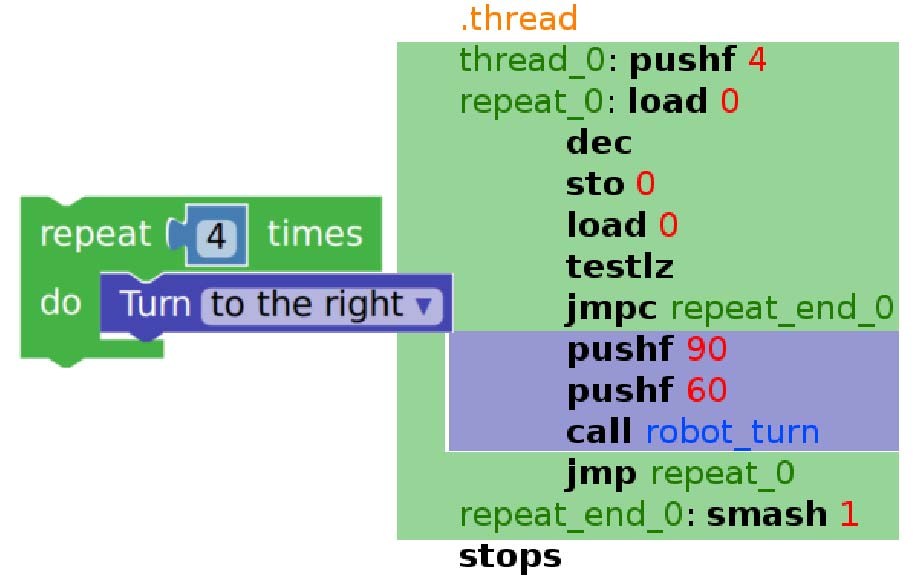
\includegraphics[width=.9\columnwidth]{metabotsample.jpg}
      \caption{Example of \metabot's visual notation (left), together with generated assembler code (right) for it (from\,\cite{Passault2016})}
      \label{metabot}
   \end{figure}

\Figref{metabot} shows a program demonstrating the use of loop control structure with a corresponding assembler code generated\,\cite{Metabot,Passault2016}.

\parhead{\marty} is a Scratch-based environment for the marty robot. The environment has also customized python to martypy. It is a collection of code that abstracts key robot functions, making it high level for robotic programming as shown in \figref{scratch-marty}\,\cite{Marty}. 

\begin{figure}[t]
     \centering
    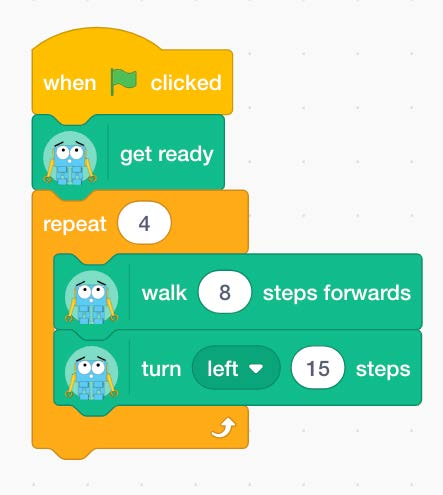
\includegraphics[width=.6\columnwidth]{ScratchMarty.jpg}
      \caption{Scratch for the robot Marty\,\cite{Marty} }
      \label{scratch-marty}
   \end{figure}

\parhead{\tello} is also a scratch-based application that generates code in Python for the drone Tello %It provides assistance for the unique features, including the landmark maps for recognition and the skipping function between the landmark maps, and multi-machine flying formation\
\,\cite{TelloEduApp}. The environment is essentially Scratch extended with a library that imports Tello-specific blocks (mainly drone flight controls) into Scratch.

\parhead{\codelab} like most educational environments provides two variants of graphical programming; sandbox for novice programmers and constructor for advanced programmers using scratch blocks to program Cozmo robot,
%; What makes the constructor mode unique is the extra features like variables, functions and math operators\
,\cite{COZMO}.  %The graphical application runs on android phones while text programming can be done on Mac, windows and Linux machines using python.

\parhead{\lego} is a programming environment equips with tools and features to program the Lego robots, among others include Ev3, and NXT %The robots can be programmed using computers, tablets or smart phones that can run Windows, Mac, iOS, Android, and iPad
\, ~\cite{LEGO,alternativeLEGO}. %It is block based graphical notation in which each block is an icon of the function it executes.  The lego robots can also be programmed in text using python, javascript, C/C++ though these are not part of the Lego mindstorms graphical environment.

\parhead{\choregraphe} is a multi-platform desktop application, allowing you to: create animations, behaviors and dialogs, test them on a simulated robot, or directly on a real one, monitor and control your robot (NAO)\, ~\cite{choregraphe,Monceaux2009}, %The graphical interface provides a flow chart like interface in which programmer uses boxes, which are abstractions of mission concepts that are used to construct a behavior to be executed. The Python SDK can be used to directly program the NAO humanoid robot. Choregraphe's box libraries provide pre-program behaviors of the robot, work area for specifying missions and simulation window for the NAO robot
\,\cite{Miskam2014} as shown in \figref{fig:choregraphe}.
%Choregraphe as a graphical environments supports robot control, behavior specification and access to sensor data for NAO robot ~\cite{Miskam2014}. 

\parhead{\blocklyprop} is a blockly based environment for specifying missions for ActivityBot robot manufactured by parallax %It is a web based environment with a client interface that can be used to connect the robot to the computer
\,\cite{Parallax}.

\parhead{\ozoblockly} is a blockly-based visual programming environment\,\cite{ozobot} with five levels of complexity ranging from icon based blocks to advanced programming level, which offers low level control functions and advanced programming features for programming ozobot.% https://ozoblockly.com/ last accessed 17th April 2019. 
 
\parhead{\minibloq} is a graphical environment for programming arduino robots like sparki, using icon based blocks, %The environment is suited for kids from age four who are still learning to read/write and any person who has never been introduced to programming 
~\cite{miniBloq}. %As an open source environment, more work is been done to accommodate advanced programmers.
  
\parhead{\turtlebot} has been championed by Dabit industries, the distributors of ROS based turtlebot3 to enable novice programmers to quickly program the turtle bot%This is motivated by blockly's drag and drop feature, which has proved friendly in end-user programming
\,\cite{turtlebot3blockly}. It provides a Blockly-based visual syntax and generates Python code for the turtle bot. %So far, Turtlebot3blockly supports two variants of turtlebot3, Waffle and Burger. 
 
\parhead{\makecode} provides a block-based visual editor and JavaScript based text editor for programming Lego Ev3 robot, %JavaScript code is generated from the visual program, which can be downloaded to the computer to which the Lego robot is connected. Makecode is a platform managed by Microsoft to provide learning environment for programming. The environment provides a simulator for the supported robots
\,\cite{makecode}.
 
\parhead{\scratchev} is a customized version\,\cite{scratchEv3} of Scratch for Lego Mindstorms Eve3, WeDo, and Micro:bit robots. %As a web-based environment, you are expected to connect the robot to the computer to download and transfer the program to the robot for execution.

\parhead{\enchanting} is another Scratch-based environment for programming Lego Mindstorm NXT robot by novice programmers (children)% The latest version was released in 2014
\,\cite{enchanting}.% Enchanting allows the programmer to focus more on the end-user domain model, as its rich visual environment enables the user easily specify the mission for NXT robot.

\parhead{\easyc} provides a graphical, wizard-like interface with drag-drop support for specifying missions for VEX robots%.  The programs are built as flow chart themes in which building blocks are icons of functional units of the program
\,\cite{EasyC}. %It is tailored for students and teachers with basic programming skills, though it still provides organic C for advanced programmers.
%http://www.intelitek.com/engineering/easyc/ last accessed on 18th April 2019.


\parhead{\robotc} provides an easy ascent from graphical to text programming  by starting with a RobotC graphical, which provides a mix of graphical blocks with natural language expressions for beginners%. For those with familiarity with programming environments, yet not ready for syntax details of C language, can use RobotC natural language, where expression are in natural language, though using text. For advanced C programmers, RobotC gives high level of abstraction for robot controllers to ease programming experience, yet providing opportunity for creating new controllers
\,\cite{robotc}.
%http://help.robotc.net/WebHelpMindstorms/index.htm  last accessed on 18th April 2019.
%\end{comment}
\newcommand{\f}[1]{\textsf{#1}\xspace}

\newcommand{\flanguage}{\f{Language}}

\newcommand{\feditor}{\f{Editor}}
\newcommand{\fsimulator}{\f{Simulator}}
\newcommand{\fdebugging}{\f{Debugging}}
\newcommand{\fspectime}{\f{SpecificationTime}}
\newcommand{\fdeployment}{\f{MissionDeployment}}
\newcommand{\fmultilang}{\f{MultiLanguageSupport}}


\newcommand{\fsemantics}{\f{Semantics}}
\newcommand{\fnotation}{\f{Notation}}
\newcommand{\flangparadigm}{\f{LanguageParadigm}}
\newcommand{\fextensibility}{\f{Extensibility}}

\newcommand{\flangconcepts}{\f{LanguageConcepts}}


\newcommand{\fflowchart}{\f{FlowChart}}
\newcommand{\fblockly}{\f{Blockly}}


\section{Design Space}

\Figref{fig:featuremodel} shows the general structure of the features we identified in our environments. 
We classified the key, top-level features into (\secref{sec:envfeatures}) capabilities and characteristics of the environments, represented by the features \feditor, \fsimulator, \fdebugging, \fspectime, \fdeployment, and \fmultilang; into (\secref{sec:langcharacteristics}) general language characteristics, represented by the feature \flanguage; and into (\secref{sec:langconcepts}) the actual concepts the languages offer to specify missions, represented by the feature \flangconcepts.
%\claudio{
%How many features have been identified in total? How many optional etc?
%How many features were identified in he brainstorming meeting? How many features were extracted from other sources?}
%\claudio{What is a general language feature? what is a Language concept?}
%\claudio{What are you going to discuss in the next two sections?}


\subsection{Specification Environment Features}\label{sec:envfeatures}
\noindent
We identified the following distinguishing environment characteristics that are related to the specification of missions.
%The value in brackets indicates the number of environments offering the optional feature out of 29. While simulator (10/29), multiLanguageSupport (13/29) and debugging (13/29) features are optional. Much as it is desirable to have to have a debugger and a simulator, not all the environments supported these features. 

\begin{figure}[t]
     \centering
    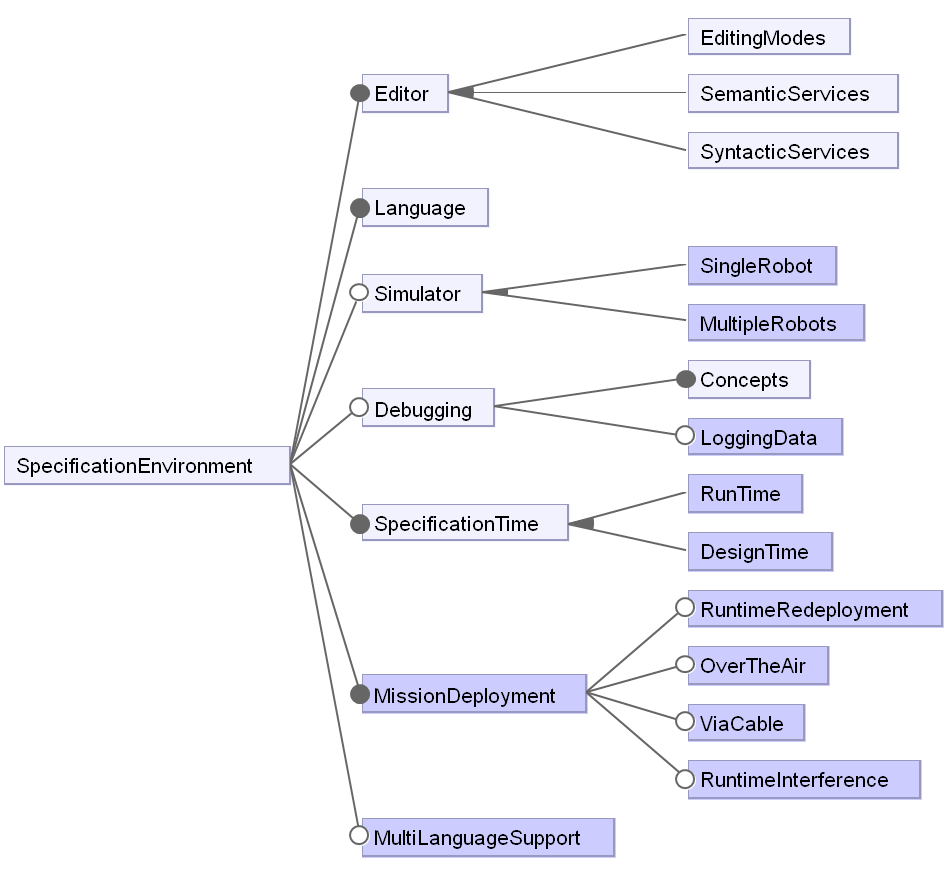
\includegraphics[width=\columnwidth]{fig/toplevelfeatures.png}
		  \smash{\begin{minipage}{8.3cm}
						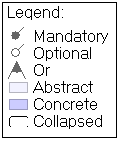
\includegraphics[width=.18\columnwidth]{fig/legend.png}
						\vspace{2.3cm}
						\end{minipage}
			}
			\vspace{-.3cm}
      \caption{Overview of all features identified%\tb{was my version, please update, but please fix the naming of some features as I did in this figure}
      }
      \label{fig:featuremodel}
			\vspace{-.4cm}
\end{figure}

\newcommand{\fsyntacticservices}{\f{SyntacticServices}}
\newcommand{\fsemanticservices}{\f{SemanticServices}}
\newcommand{\feditingmode}{\f{EditingMode}}

\parhead{\feditor.} While the editor tooling in our environments of course offers typical editor capabilities (e.g., copy, paste or undo), we found the following distinguishing characteristics represented by the features \fsyntacticservices, \fsemanticservices, and \feditingmode, as follows.

%Besides the basic editor features such as cut, paste, and redo; we also found syntactic services, semantic services, and editing modes as editor features.

Syntactic services (feature \fsyntacticservices) support developers creating a correct abstract syntax tree (AST) of the mission specification, according to the language's abstract syntax. We found various of such services. Especially syntax highlighting with coloring is available in all environments.  %todo: verify \flyaq and \tivipe
We furthermore found a range of convenience services, such as an outline view for navigation support (e.g., in \picaxe), syntactic completion templates for users (e.g., in \edison and \ardublockly), and automated formatting (e.g., in \arcbotics, \robotmesh, and \vex).

%and invalid variable name \minibloq -> isn't that a kind of error highlighting?

%restructuring, aligning or lay-outing \cite{erdweg2013languageworkbenches} as seen in \robotmesh, \vex  -> explain what that is (didn't find in the spreadsheet)

%offer support for correct expression structure, as defined by a language to support specification of missions. The syntactic services captured include; language specific syntax coloring and symbol shapes in graphical notations, were evident in almost all the environments studied with exception of \flyaq and \tivipe where the authors were not sure. -> symbol shapes is not a syntactic service

Semantic services (feature \fsemanticservices) support developers creating an abstract syntax tree that is semantically meaningful, inspired by the definition of semantic services in~\citet{erdweg2013languageworkbenches}. We identified: auto-completion (e.g., in \vex, \trik, \picaxe, \edison);  live translation where generated code is displayed side-by-side to the graphical notation (e.g., in \easyc); error highlighting (e.g., in \edison, \aseba, \vex, \robotmesh, \blocklyprop, \minibloq, and \easyc) directly on the mission specification, for instance the indication of compile errors at the respective lines in \blocklyprop, or as a pop-up help (e.g., in \edison, \missionlab, and \choregraphe). However, more than half of the environments did not offer any semantic services. % -> verify

%and auto-help when activated enables automatic reference when blocks are selected ~\cite{ozobot} as seen in \ozoblockly, \edison.

Finally, the editing mode (feature \feditingmode) typically classifies into parser-based and projectional editing\,\cite{voelter2014projectional,berger2016pe}. In the former, the user edits the source code, which is represented by a sequence of characters in a free form. In the latter, the user's editing gestures directly change the underlying AST, which is projected using projection rules into a user-observable syntax, which can resemble textual and visual syntax, or a combination of both. \Figref{fig:easyc-sidebyside} illustrates the power of projectional editing in the environment \easyc, showing visual and textual syntax side-by-side. The typical continuous enforcement of a correct AST in projectional editing guides users towards correct mission specifications, which can also be seen as a semantic service. For all our environments, given the restriction to visual languages, every environment provides a projectional editor. However, four also offer textual languages, to be used in parallel as an alternative, relying on parser-based editing: \aseba, \vex, \turtlebot and \robotc.

\parhead{\fmultilang.} A total of 13 of our environments offer multiple languages to specify missions. While at least one visual language is supported (according to our selection criteria), many environments offer at least one more language. For instance, \picaxe provides two visual languages, based on a \fflowchart and a \fblockly notation, respectively, as well as it offers the general-purpose languages Basic and Javascript.


%, and projectional mode where, the program has a standard fixed layout. In projectional editors are structured editors in which a developer works directly on the bstract syntax tree(AST) \cite{berger2016pe}, coding is done using intuitive onscreen visuals.
%\parheadit{Example} Of the 29 environment studied, only four support parser based editing mode; \aseba, \vex, \turtlebot and \robotc. This finding is not surprising since in the selection criteria, the study is biased to end-user supporting environments. 

\parhead{\fsimulator.} Ten of our environments provide simulation support to test missions before they are executed. This helps in ensuring safety and creating opportunities to train users without necessarily using the actual robots. One of the simulators, that of \missionlab, even supports multiple robots.
%The simulator either support single robot at a time or more than one robot and/or robot type. -> which ones? do we have evidence that multiple robots are supported by at least one simulator?

\parhead{\fdebugging.} A total of 13 of our environments offer debugging support. We found a variety of debugging tools, including the live monitoring of sensor data, the state of actuators, and variables in the environments \picaxe, \aseba, \trik, \flyaq, \easyc, and \edison. The environment \edison offers a box to control inputs, manipulate data, and monitor the use of variables. % -> what was 'bug-box'?
Interestingly, \makecode communicates execution traces via sound and printing text between the execution of program blocks. % -> not so clear
We also found the typical break-point mechanism to hold and monitoring executions (e.g., in \robotmesh).
Furthermore, \openroberta provides a 'check' menu to confirm that the mission specification the robot's configuration matches---important since the environment supports different types of robots. 
% -> this all needs to be verified

\parhead{\fspectime.} Missions are specified either at design time or run-time. Design-time specification provides all the details about the mission before the execution starts.
 %which calls for explicit modeling of the environment.
All our environments support design-time specification. A few environments (\turtlebot, \sphero, and \choregraphe), however, also offer some remote-control functionality to intercept the mission execution at runtime. % -> verify
%with the exception of \turtlebot, \sphero and \choregraphe. For instance, in \choregraphe, different missions can be deployed on the robot at run-time. \sphero supports interaction with the robot at run-time using a Bluetooth connection. % -> I think this is wrong

\parhead{\fdeployment.} Missions, once specified, are transferred to the robots for execution. Not surprisingly, we found different combinations of media to transfer missions, including USB cable, Ethernet cable, custom cable, as well as WiFi and Bluetooth connections.
 %Environments such as \trik and \lego support USB, WiFi, and Bluetooth connections for deployment over-the-air. While \tello missions can be deployed using Bluetooth, and Wi-Fi. Most environments use either USB, Ethernet or a custom cable to deploy missions to robots. \\ 


% \textbf{items removed}
% \begin{itemize}
%     %\item file access
%     \item time has been merged as a measure of action under action types
%     \item example as an example of syntax services
%     \item formal notation (generic code, natural language text, forms, blocks, icons) and secondary notation (syntax highlighting, size, notation color, comments) as concrete features of notation.
%     \item behavior concepts with concrete features like discrete behavior and continuous behavior from language features
%     \item robot with single/multi-robot mission (swarm/team), multi-robot, single robot, robot types and connection and multi-robot types as concrete features
%     \item Mission deployment support; hardware requirements and software requirements
%     \item debugging environments; simulation, actual robot
%     \item modeling concepts and explicit modeling of environment 
% \end{itemize}





	
\subsection{General Language Characteristics}\label{sec:langcharacteristics}
As illustrated in \figref{fig:languagefeatures}, we identified the following general characteristics in which the languages differ, represented by the features: \fnotation, \fsemantics, \flangparadigm, and \fextensibility. The actual concepts offered by the languages will be discussed in \secref{sec:langconcepts}.

%The language constructs for motor, and sensor  data configurations are abstracted closer to those who are familiar to the use of the sensor than just robot engineers. For example \emph{set motor speed, obstacle detector event block (grey: ignore detector, white: object close and black: object far)}. \claudio{The previous sentences are part of the methodology} The fact that these languages support graphical notations breaks the barrier created by text notation among novice programmers, as asserted by Fernandez-Permomo et al.\cite{Fernandez-Perdomo2010}, hence increasing usability, learnability and satisfaction among end-users. \claudio{Not clear what is the point of this sentence? Here we should discuss the FM we have created}
%\tb{we need examples of domain-specific terminology in the languages, can you provide some? also, examples why you think the languages are end-user facing; why is that the case?}
%For instance, they support end users through \dots. Most (X\,\%) are also graphical.
%domain, which generalized features that support novice programmers and robotics domain, which take care of technical features for professionals in robotics or software engineering.
All the languages identified in the environments including the textual ones have been customized to support the robotics domain, for example by introducing domain specific actions. Some of the actions in \lego are stop motors, play tone in \trik, set robot's state, set top color in \aseba,  drive straight, and turn right. %in \lego are some domain specific actions.% \tb{how? give examples of domain-specific keywords and domain-specific graphical elements}.

\begin{figure}[t]
     \centering
    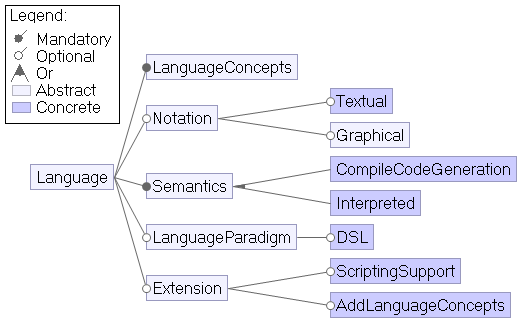
\includegraphics[width=\columnwidth]{Languagefeatures.png}
      \caption{Language Characteristics}
      \label{fig:languagefeatures}
   \end{figure}

\parhead{\fnotation.} All our environments offer languages with a domain-specific visual notation (concrete syntax) for end users. For instance, a block \emph{Motor forward} in \trik has a gear icon with a forward arrow depicting a forward-running motor. The user only specifies the motor power and the port in which the motor connects. 13 of our environments additionally offer a textual syntax
%\tb{do you know for how many the textual syntax belongs to the same language (the main, visual language) and for how many it is a separate language (which could also be a gpl)?}.

\begin{itemize}
	\item Graph-based
	\item 
\end{itemize}

The notation found is: (i) Blockly-based as shown in Figure \ref{metabot}, (ii) Scratch-based as shown in Figure
	\ref{scratch-marty}, (iii) forms and tables as shown in Figure \ref{fig:robotcgraphical}, or (iv) textual where End-user codes a mission using text characters.

%\tb{but thought we have graph-based and block-based as our features?}
%\begin{itemize}
%	\item Blockly-based as shown in figure \ref{metabot}%\tb{characterize what you've seen; how does it look like}
%	\item Scratch-based as shown in figure
%	\ref{scratch-marty}%\tb{characterize what you've seen; how does it look like}
%	\item forms and tables as shown in figure \ref{fig:robotcgraphical}%\tb{characterize what you've seen; how does it look like}
%	\item textual where End-user codes a mission using text characters.%\tb{characterize what you've seen; what kinds of textual notations do we have? how do they look like?}
%\end{itemize}

Some of the graphical notations used blocks, which are directly connected to each other for instance \trik, blockly, and scratch based languages. While \choregraphe, Flowol in \robotmesh, and flowchat in \picaxe use connectors between blocks to form graph like structures. %A graphical notation is either block-based or graph-based. A block-based \tb{what's the difference? briefly describe}.
Interestingly, \flyaq offers a map-based 
%\tb{so, is that classified as graph-based or block-based, or sth. else?} 
monitoring mission language to specify missions by clicking on locations where tasks will be executed. 

The textual or visual notations offered by the respective environments are summarized in the Table \ref{notation}. Some environments use a mix of textual and visual notations, like \easyc, as shown in \figref{fig:easyc-sidebyside}, or make use of tables and forms, as \robotc as shown in  %\figref{fig:robotctextual} and 
\figref{fig:robotcgraphical}.

%Textual: \edison, \choregraphe, 
%%\tb{choregraphe is definitely visual!},\swaib{the point is it also supports textual notations} 
%visual: \minibloq, \trik, \choregraphe, and mix of both text and visual \easyc \figref{fig:easyc-sidebyside} or by use of tables and forms as provided by \robotc in  %\figref{fig:robotctextual} and 
%\figref{fig:robotcgraphical}. % \tb{add screenshot}.
%The notations offered by the respective environments have been summarized in the table \ref{notation}.

%- symbol shapes in graphical notations
%- Blockly library: It has been implemented in various environments as shown in table \ref{notation}% Roberta\,\cite{OpenRoberta,PICAXE,RobotMeshStudio} \tb{make complete, where else?}

\begin{figure}[t]
	\centering
	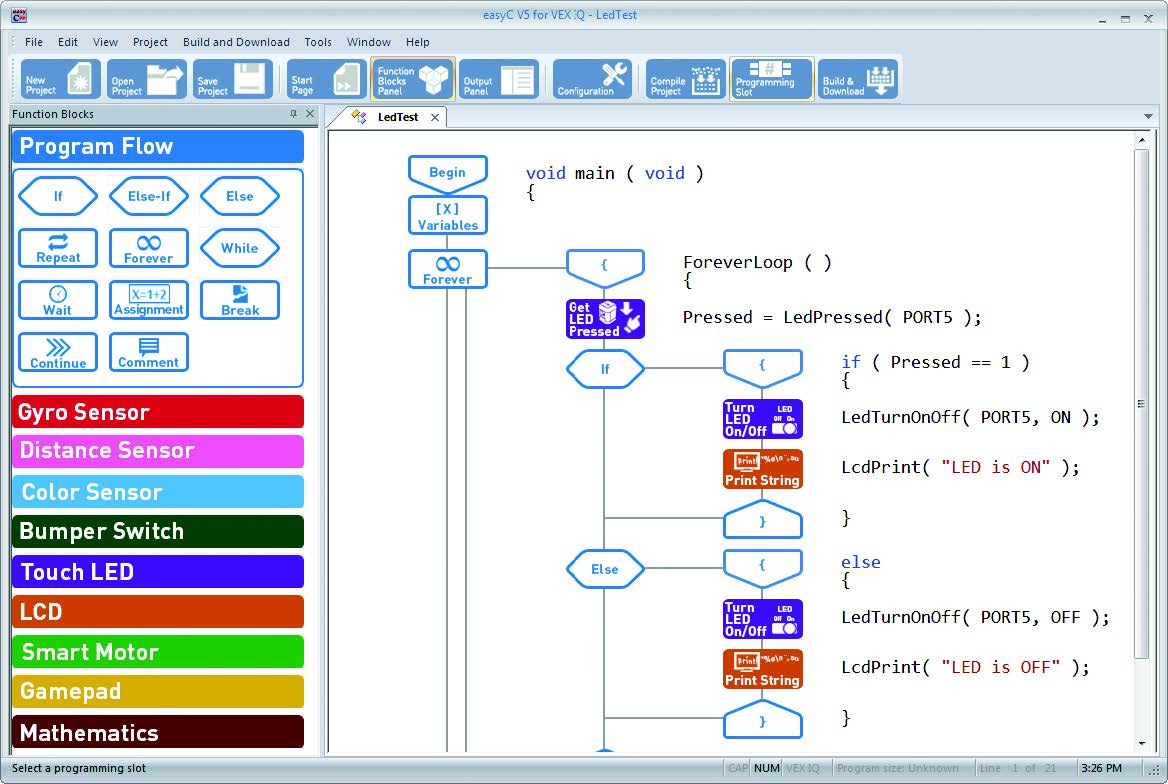
\includegraphics[max size={0.5\textwidth}{\textheight}]{projectionalEasyC.jpg}
	\caption{Graphical and textual syntax side-by-side in \easyc's projectional editor%\tb{TODO: create better screenshot}
	}\label{fig:easyc-sidebyside}
\end{figure}

% \begin{figure}[t]
% 	\centering
% 		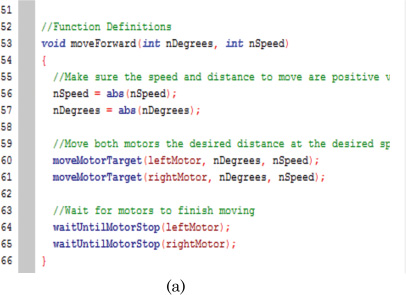
\includegraphics[max size={0.5\textwidth}{\textheight}]{robotCtext.png}
% 	\caption{RobotC, (a) textual \cite{Schunn2017} }
% 	\label{fig:robotctextual}
% \end{figure}

\begin{figure}[t]
	\centering
		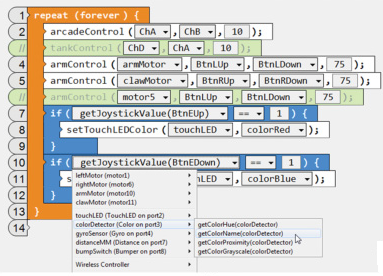
\includegraphics[width=\columnwidth]{robotCgraphical.png}	\caption{\robotc, graphical notation (from \cite{Schunn2017}) }
	\label{fig:robotcgraphical}
\end{figure}
%\claudio{Missing verb. Which details?} %Secondary notation services provide extra information on the marks and cues used for specification of missions, like; comments, and size of blocks~\cite{Blackwell2001}.

\begin{table*}
\caption{Kinds of notation supported by the environments (the graphical notations belongs to the primary DSLs of the environments; the textual ones to additional languages supported, which can be a GPL)}
\label{notation}
\begin{tabular}{ m{3cm}m{13.6cm}}
\toprule
\textsf{notation} &\textsf{environment}\\
\midrule
\textbf{graphical} &\\
Blockly-based & \picaxe, \ardublockly, \openroberta, \arcbotics, \aseba, \robotmesh, \blocklyprop, \ozoblockly, \turtlebot, \makecode, \robotc \\
Scratch-based & \edison, \aseba, \sphero, \vex (modkit), \marty, \makeblock, \codelab, \tello, \scratchev, \enchanting, \\
Control-flow graph & \picaxe (flow chart), \missionlab, \tivipe, \choregraphe (flow diagram), \robotmesh (flowol), \trik \\
Custom & \edison(EdBlock), \flyaq (map), \aseba(custom blocks with icons, see \figref{fig:aseba-vpl}), \codelab (icons), \lego(icons), \minibloq(icons), \easyc\\
\midrule
\textbf{textual}&\\
C/C++ & \arcbotics, \vex, \robotmesh, \trik, \easyc\\
Python & \edison, \robotmesh, \marty, \makeblock, \trik, \codelab\\
%Java & \patrizio{empty here? Remove?}\\
JavaScript & \picaxe, \sphero, \marty, \trik \\
Custom & \picaxe (custom language in the style of Basic), \ardublockly (Arduino C), \aseba (custom event-based language) \\
\bottomrule
\end{tabular}
\end{table*}



\parhead{\fsemantics} The semantics of our languages are determined by either interpretation or compilation (target code generation). The mission specified is either semantically translated (compiled) as shown in \tabref{Codegeneration} \patrizio{missing table} or interpreted to preserve what is specified and what the robot actually executes. Apart from \lego, and \codelab whose missions are interpreted, all the other 27 environments generate code. \metabot generates assembly code while the rest compile generated code before robot executes the mission.\patrizio{check this sentence. who are other? What do we want to say?}  \trik supports Lego Ev3, Lego NXT, pioneer kit, and the TRIK robot, even though the environment does not cross-compile as missions are robot specific. In the case of Lego EV3, missions are interpreted, with support for both USB and Bluetooth connections.
%\tb{this has nothing to do with semantics}. 
In the case of Lego NXT, besides interpretation, \trik generates Russian C language and NXT OSEK C language, while in the case of TRIK robot, the environment generates Java Script, PascalABC, Python, and F\#.%\tb{why does it generate programs in so many different languages?} \swaib{Russian C, OSEK C are target languages seen in the list, however there is no much documentation about them in the tool documents. I have not figured out why TRI robot missions can be generated into several languages}. \codelab provides support for mission interpretation using Python SDK\tb{unclear, what does that mean?} \swaib{the interpreter was built using python software development kit (SDK)}.

%\tb{I just checked \choregraphe, and it does not generate .NET bytecode (which would be MSIL), but it provides language bindings (an API) for .NET so that .NET programs can call API functions of NAO to control it}

%\tb{what about all the other environments?} \swaib{cross examining the data collect can help in fixing such gaps}


\parhead{\fextensibility} -
Some environments provide features for extending the language with new concepts. We classified such abstract features into two concrete features ScriptingSupport and AddLanguageConcepts. %{ can be in form of scripting support, editing graphical programming blocks or adding new language concepts using the generic language of the environment} \claudio{Check that abstract features and concreted features are defined somewhere}.
ScriptingSupport allows the creation and launching of new scripts created to handle new language constructs. This is the case for instance of the creation of  movements for NOA robot in \choregraphe.
 While AddLanguageConcepts support allows user to edit and create new blocks, for example myblock in \makeblock, creating new blocks in \tivipe, extending monitoring mission language in \flyaq. \patrizio{I don't understand the previous sentence}  Open source environments use github for communities to continuously extend the language feature e.g.: \sphero, \openroberta, and \flyaq. Environments like \easyc, \flyaq, and \missionlab provide opportunity to extend the language features using \ugh{the generic languages, not necessarily scripting or editing graphical blocks}. \patrizio{this is not clear}
%\claudio{How is this info related with the FM?} \swaib{Extension is a feature in the FM} 
\lego extends the language features by importing custom programming blocks from vendors which manufacture sensing blocks compatible with the Lego brick. However, most commercial environments, extensions  are done by the commercial companies. E.g.: \arcbotics, \edison, \blocklyprop, \vex, \robotmesh among others.

\parhead{\flangparadigm} - All our languages are DSLs as opposed to general-purpose languages (GPLs), since all incorporate keywords representing concepts pertaining to the robotics domain. However, some language also offer GPLs for programmers, in addition to their primary visual DSLs.
%defines the category of languages found in the specification environments. All languages in the selected environments are domain specific languages with a bias to robotics and software engineering domains. In the interest of end-user programming, it is desirable to see languages whose DSLs are specific to user domains like farming, or environmental management.% \claudio{What were the options? Is it really a feature?}



\subsection{Language Concepts}\label{sec:langconcepts}
Language concepts is a sub-feature of languages that %is treated separately because it 
highlights the concepts that determine the expressiveness of the language while specifying missions. Sub-features of the language concepts include: control flow, modularity of the language, variable data types supported, event support ability, the types of sensor data that can be read, control flow paradigm, actions the robots can perform, exception handling, file access feature, function libraries, and multithreading support.

%\claudio{Concept never introduced. What is a concept? Move the following line somewhere before.}
Language concepts is a feature %are features 
used by  end-users to express missions. 
%\claudio{How are concepts and features related?}
The expressive power of the environments is determined by the language concepts that are salient to the end-user. As shown in \figref{fig:langconcepts}, we categorized these concepts into control flow, modularity concepts, variable data types, event support, read sensor, control flow paradigms, actions, exception handling, file access, function  library, and multi-threading.  

\begin{figure}[t]
     \centering
    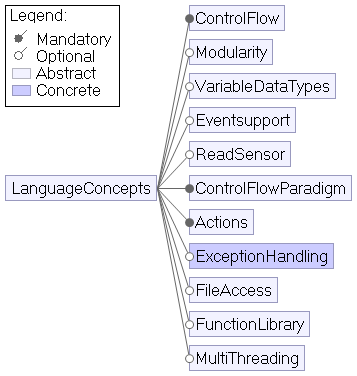
\includegraphics[width=\columnwidth]{LanguageConcepts.png}
      \caption{Language Concepts}
      \label{fig:langconcepts}
   \end{figure}

\parhead{Control Flow} - The languages typically offer several kinds of control-flow statements, such as, conditional structures (\texttt{if-do, if, if-else} and switch) loops (\texttt{do-while, while, forever, repeat while, repeat until}), and  interrupts (\texttt{loop interrupt} in \lego, \texttt{stop all} in \tello, \texttt{wait (time/event), break, and until}).
%\claudio{Use special font, e.g., texttt}
Multi-threading controls might be found also in \trik (\texttt{fork, join, kill thread}) and in  \lego for running tasks simultaneously (\texttt{sequence plug exit}).

\parhead{Modularity} - Modularity focuses at mission sub-components that are used to accomplish specific tasks.
Examples include \metabot, \ardublockly, \openroberta, \choregraphe, \sphero, \robotmesh, \metabot, \makeblock, \ozoblockly, and \turtlebot; they create mission modules using functions and function calls. Choregraphe implements robot behaviors as boxes, which are connected in a flow chart to form a mission. \lego imports blocks from external environments that are compatible with \lego. \trik implements subprograms, functions, and module with symbolic icon of what these components do; in this way they become mission modules. \picaxe implements procedures of particular concepts, which then can be invoked and used.  \missionlab has predefined states used to build a state machine for a given mission. 

\parhead{Variable data types} - While \flyaq, \missionlab, \tivipe, and \trik do not have exclusive variable data types, the rest of the environments have primitive types and compound data types. The primitive types include integer, decimal, character, float, number, and boolean, while compound types include strings/text, arrays, table, and lists. Other types include sound in \ozoblockly, logic (true, false) in \lego, degrees in \tello, and color in \sphero. In \aseba, state is a variable type;  for instance temperature is a variable that can take values like off, low, medium, high, and light is a variable that can take values like on and off. 

\parhead{Function libraries} - Function libraries offer functions and operation on data, including complex algorithms used to process data. Most environments provide function libraries for mathematics, logic and string operation; however \missionlab, \flyaq, \aseba, \codelab, and \tello do not offer such libraries. 

%\parheadit{Examples}
Top provide some examples, the logic functions include comparison like and/or, not, true/false, null, and test. The math sub-feature includes mathematics function, calculating parameters, trigonometric function, constant, number property, change by x, round, list evaluation, remainder of, constrain, random (integer, fraction), squareroot, return constant(sqrt, pi,...), sum of list, array operations, and range. Text operations include create, append, build string, length, find occurrence in a list, get sublist, is empty, get letter, get substring, join, and letter 1 of.  %Math box and data edit box in \choregraphe.     

\parhead{Control flow paradigm} - This determines how missions are executed, which can take the form of imperative execution, reactive paradigm or goal based. In imperative execution, the mission runs in the order of sequence of the tasks specified, which is the common paradigm of most environments in this study. However, \aseba Visual Programming features a reactive paradigm in which events, which act as triggers are matched with corresponding actions, which categorize it as a reactive. In some of the imperative environments like \picaxe, reactive aspects are also realized as robot, which responds to sensor data during mission execution. We did not come across an environment, which follows a goal-based control-flow paradigm.

 
\parhead{Actions} - These are activities robots execute to achieve a given task. Some are reactions to events, while others are activities that are imperatively specified in the mission. We classified robot actions as action type, actuation action, communication action, and movement actions. Robot actions  can be instantaneous actions e.g. take photo~\cite{FLYAQ}, pause, resume~\cite{PICAXE}, or continuous action e.g. follow line~\cite{LEGO,Sphero}, or timed executions where duration of execution is measured with start/stop time or events, like record a video~\cite{FLYAQ}. The actuation actions refer to device/actuator wise actions like grasp an object, motor movements, audio play. Communication actions include interacting with humans and non-human agents.  Communication with humans can be of the form of text, video, or audio. While non-human agents can  be categorized as tuple space, publish-subscribe or message passing. Tuple space is a shared space where shared data items are kept for access to entities entitled to access them, publish-subscribe where publishers avail messages regardless of receivers while subscribers receive messages they have subscribed to.
Movement actions manage mobility of robots. Languages offer concepts that specify how a robot moves from one location to another. Such  concepts are either absolute ``map coordinates", or relative like direction, distance, or travel time.\\
%\parheadit{Actuation examples identified} - 

Actuation examples include get button code, play tones, sound, stop motors, clear encoder, angular servo, turn on LED, detection with videocamera, line detector, video streaming enabling, beep note, buzzer, display, status light, object observation, taping, face status (smile, frown), lift, backpack, speak, think, change color, hide number, change volume, screen print, screen draw(line/object), start timer, set robot state, say hello, stand-up, wave with hand, move, DoPhoto, monitor street (road task), Intercept Object, LeaveRoom, Localize position, LookForObject, MarkNearestObject, MarkNearestDoor, MoveAhead, MoveAway, MOveForward, MoveToward, PickUp, SurveryRoom, Talk, Terminate, TrackTarget, Wait, Wander, follow line, gripper(open, close, stop), set mode(active, rest, sit). \patrizio{not sure we need all this}\\ 
 
%\parheadit{Action type examples}
Action type examples include the ``random eyes duration ms" block that is used in \openroberta to turn NAO's eye LEDS to change eye color for specified duration in milliseconds. Instead in NXT the ``get value ms timer" block is used as a sensor to read current time for another block, while the ``reset timer" block is used to reset the internal timer to zero. Similar time constructs also exist in other environment, like the wait time and elapsed time blocks in \ardublockly, the set roll time in seconds as a variable, time elapsed, get current time, set timeout, set time interval in \sphero, the set timer(seconds), timer, wait(seconds), wait until (event) in \vex among others. \\

%\parheadit{Communication examples} 
Communication example include infrared messages exchanged among robots in  \edison, \lego, and \openroberta, and Bluetooth messages exchange between bricks in Lego Ev3. In \missionlab, when in GOTO state, robots share information about target goal position and map of the environment among each other directly or through broadcasts. \sphero, \vex, \makeblock, and \tello broadcast message between robots. \flyaq supports synchronization and communication messaging among drones at run time.  \trik supports sending message to other robots. For what concerns human and central system to robot communications, examples are hand-clap and touch in \aseba, and \enchanting, send text, send number, send command, receive character, send character, send, and receive message in \tello, speak short phrase in \codelab, say text in \trik, \tivipe from the robot to the environment. In \choregraphe robot can share text with humans. In \arcbotics, humans interact with robot through beep, status led colors, infrared remote code and \picaxe communicates through infrared messages. Eleven of the 29 environments do not offer any communication language constructs. \\

%\parheadit{Movement examples} 
Few of the environments support absolute movement actions, such as e.g. goto (coordinates) in \flyaq, \missionlab, \makeblock, moveto (coordinates), movefast (coordinates, duration) in \tivipe, roll(angle, speed, time), spin(angle, time in seconds) in \sphero, drive (distance) in \codelab. For relative movements we mention go/move/drive/turn/fly (forward/backward/left/right/room) as seen in most of the environments like \metabot, \trik, and \lego.

\parhead{Event support} - Event support considers language abilities to handle events like creating event handlers, the types of events that can be recognized, and mechanisms of synchronizing events to subsequent actions. The common language constructs for event support identified include when (event), when (event) do, wait for (event), wait until (event), wait (event), on (event), capture(event), move until (event), broadcast and wait 9event) in \vex, AtGoal, AtEndOfHall, in \missionlab, and delay (event). The events are sensory data that trigger the next robot action. However environments like \arcbotics, \tivipe, \minibloq, \turtlebot, and \robotc do not have event support language constructs.\\

\parhead{Read Sensor} - From the environment the robot captures data through sensor readings, which inform robots next action. Much as most environments offered language support to capture respective sensor data, \turtlebot and \missionlab do not offer language concepts to manipulate sensors while \choregraphe supports vision recognition using vision reco box and sound recognition using speech reco box. \ozoblockly uses proximity sensor concept to detect objects without details of the sensor.\\

%\parheadit{Example} 
Common sensors captured in the environments include gyro for measuring rotations, light/light intensity, sound/clap detector, touch, temperature/thermometer, ultrasonic for measuring distance, timer, compass, accelerometer, gesture detector, and face recognizer. Other sensors are sonar, infrared ranger, GPS module, finger print scanner, motor rotation counter, energy meter, line detector, angle reader, line tracker, potentiometer, velocity, power(wats), current (amps), magnetometer, and force resister. The number of sensors on the robot and nature of the missions the robot is designed for determine the language constructs for the sensors.  \\

\parhead{Exception Handling} - Only three environments, namely \openroberta, \choregraphe, and \codelab offer support for exception handling in their text notation but none in the graphical notation. %\tb{probably just very few, right?} 

%\parheadit{Examples} 
More specifically, \openroberta exploits the Python exception handler, and \choregraphe exploits the try catch block for all errors in C++ software development kit (SDK) and the try catch block for face detection error in python SDK. \codelab offer support for exception handling for the following errors: actionerror, animations not loaded, can not place objects on this, connection aborted, connection check failed, connection error, no devices found, not pickupable, and robot busy.\\

\parhead{File Access} - It is a block found in \lego, used for reading and writing data from and to memory, close or delete a file. Such file can record for instance ambient light measurements taken at given time intervals, which are stored in memory and can be displayed on the LCD display screen ~\cite{LEGO}. \trik allows writing to robot file system, \choregraphe supports open, close and save operations to file while \missionlab offers read, write, close and delete language construct for file operations. \picaxe also supports read and write operations. The rest of the environments do not offer any language support for file access operations.

\parhead{Multithreading} - This concept when supported by a language enables users to do several activities without waiting for one activity to end. This improves speed of execution especially when it involves user. In \robotmesh,  using blockly editor,  \textit{start} block creates s thread, \textit{sleep} for x seconds forces thread to \textit{yield}, \textit{start autonomous} creates a thread that runs in autonomous mode of the robot, \textit{start driver} creates a thread that runs in driver mode. In python, sys.run\_in\_thread(f), sys.thread\_id(), sys.sleep(t). In C++, thread (void (*callback)(void)), get\_id(), join(), interrupt(), yield(), sleep\_for(unit32\_t time\_ms), lock(), try\_lock(), unlock(). \trik offers fork, join, kill thread, send message to thread functions to execute multithreading. \lego offers Sequence Plug Exit block for creating parallel tasks, though the simultaneous tasks need to be manually verified to avoid resource conflicts. \makecode and \robotc use \textit{run in parallel} block to support multithreading of mission tasks. \tivipe uses \textit{splitSCIS} to split and run three modules  in parallel. \missionlab supports Cthread, which is a lightweight process threads package from Georgia Tech which operates under Linux, SunOS operating systems. While \picaxe supports multi-tasking with operations like; restart, resume, and suspend.












  %\begin{figure}[h]
% \subsection{How the environments differ}
% \noindent
% General language features ~\cite{Clark}; notation is the concrete syntax of a language expressed either as textual syntax or visual syntax. Abstract syntax describes the vocabulary of the concept and how they are combined, while semantics describes what the language represents and means. Mapping feature describes how the language translates to other languages, its semantic equivalence, abstraction level with respect to similar languages and also internal mapping of the abstract syntax to concrete syntax as part of the language architecture. While extensibility of the language states how the language handles adding new concepts to boost its expressiveness. By considering features as end-user visible characteristics of the system, the environments can be compared based on; notation, extensibility, semantics and some aspects of mapping.
% Feature matrix\\
% $\bullet$ Notation matrix\\
% $\bullet$ coupling and reuse of mission artifacts in different contexts\\
% $\bullet$ control flow at run time; imperative (sequence and branch, in concurrent threads, reactive to events or declarative)\\
% editing features (syntax, semantic 

% What made the environments different\\
% $\bullet$ \parhead{Based on underlying technology} blockly based, scratch based, or generic \\
% $\bullet$ \parhead{Connection of blocks} flow chart based or nonflow chart (no links between blocks)\\
% $\bullet$ \parhead{Closeness of mapping} icon based or regular graphical blocks\\
% $\bullet$ \parhead{User domains} students focused (learning), electro-mechanical domain with features of electronics components like motors, programming domains demonstratting features of programming languages,\\ 
% $\bullet$ \parhead{Semantics} are the languages interpreted or compiled. The common generated code languages including; Java Script, Java, C/C++, Python.\\
% $\bullet$ \parhead{Control flow Vs Data flow based}. Control flow based languages graphical languages organize functional blocks into directed graph using arrows. A current block executes command and passes control to the next block based on the output generated. While in data flow based languages, program blocks are data variables that receive data from sensor system, whose value determines the next course of action ~\cite{Mordvinov2017}.
% ======================
% To be crosschecked~\cite{crosscheck}

% \begin{itemize}
% %In robotics, who specifies the mission requirements? (user domain expert, robotic engineer)
%     \item Task features; behavioral/functional model
%     \item Environmental features
%     \item Performance metrics; governing rules that constrain the behavior of the task
%     \item Robot capabilities; physical parts(actuators) that exhibit the behavior of the task
%     \item Mission goal; user goal, purpose of the mission
%     \item Single robot or team of robots mission, if multi-robots, the task distribution/delegation strategy (automatic or explicitly specified).This also includes interactive missions where humans work with robots.
%     \item In quantitative specifications, execution times for respective tasks should be specified otherwise sequence of specification for qualitative specifications.This can be an input to motion planning unit.
%      \item Text; type or select from drop-down list
%     \item Visual/graphical; point at locations to visit in a map, drag and drop domain primitive icons to define sequence of events.
%     \item Audio interaction with robot
%     \item task specification tree where nodes are declarative specification of tasks to perform\cite{Doherty2013}. Can missions be decomposed to tasks and subtasks to form a task forest or bigger tree? Weintrop et al \cite{Weintrop2018} reports use of trees to hierarchically program tasks. Robot routine is broken  into  a series of steps, with each step having sub steps, resulting into hierarchical program as implemented in universal robots' polyscope interface.
% \end{itemize} 
% \claudio{Can you try to put here for each RQ the concepts that aims at answering that RQ. For example, 
% RQ1: Debugging, Simulator.}
% \claudio{If you collected something that is not mapped to an RQ you have two options:
% 1 - you drop it. Because the information is not useful
% 2 - you add a new RQ.}
%\section{Discussion}
%\swaib{what environments are in literature but not captured by the study? What are the features expected but not found in the environments studied?} \tb{We might also discuss the features we think are missing or underrepresented, but this would just be a discussion, nothing for which we can define a research question that we systematically answer.}


\tb{move paragraph to S.4, give the numbers when reporting the results}
The language sub-feature, figure  \ref{fig:languagefeatures}, identifies five features from which four are mandatory: language concepts, notation, semantics and language paradigm. While the extension feature (21/29) is an optional feature. Some language support extension of the language functionalities by any user especially those which are open-source  while other do not.

\tb{move paragraph to S.4, give the numbers when reporting the results}
In Language concepts feature, figure \ref{sec:langconcepts}, we identified eleven sub-features, from which three are considered mandatory: control flow, actions and control flow paradigm . While modularity (17/29), variable data type (25/29), event support (24/29), read sensor (26/29), exception handling (3/29), file access (7/29), function library (24/29) and multithreading (8/29) are considered optional features. Without the optional features, the language can still support mission specification, however we did not find a situation where all the optional features do not exist in a particular language.

%Robotic mission describes robot behavior over time and space, as a dynamic system, where behavior is action under specified circumstances. The circumstances can be continuous like video streaming or instantaneous as states or phases of the mission. 
Most end-user programming languages provide either graphical notation or programming by demonstration. However in graphical environments, it is still hard for end-users to define new behavioral primitives.%~\cite{Bravo2018}. 
 According to Bravo et al. ~\cite{Bravo2018}, the following are some of the features expected in mission specification environments; both visual and demonstration programming abilities in specification environments, environments ability to support multiple robot mission specifications, collaborative specification environment where more than one users can concurrently specify a mission, ability for end-users to modify and or create new behavioral primitives. 
 In the environments in this study, mechatronic constructs for motor \& sensor specifications and programming constructs like control flows have reasonably matured in graphical notations, making it easy for end-users to easily program missions. However, more work is needed to match the flexibility of robot hardware to end-user domain model in farming, environmental management, personal assistance among other domains to fully achieve end-user programming in robotics. The complexity in the algorithms for programming by demonstration and the rigorous and tiring process of training the robot does not make it easy for end-user to flexibly program robot for tasks of everyday life.
%\noindent
 %Dynamic systems' behavior descriptors are time and space. It is the motion through state/phase space.
%Therefore a mobile autonomous robot mission is seen as dynamic system that interacts with its environment over time. %In an effort to understand what can be specified in a robotic mission (RQ1), the following can be considered as robot behavior parameters;
% \begin{itemize}
% \item Mission goal; to carry all cups from dining table to kitchen table
% \item Task;the primitive actions pick a cup from location A table 1, move to location B release the cup on table 2.
% \item Repeat task until [constrain] or not
% \item Constrain; time, sequence of events, number of cups, presence or absence of an object or situation,..].
% \item preconditions to start a mission or a task; readiness test
% \item Location; home, mission start/stop locations, action locations
% \item Required actuators for the actions mentioned in the task;grasp - hand, detect cup - sensor or camera.
% \item Performance indicator; user acceptance parameters or indicators
% \end{itemize}
%From the study interestingly the following where identified as mission specification parameters; ... Users can only specify at high level as robotic software engineers generate other requirements to make the mission specification complete enough for execution.
%RQ2 explores how missions are specificatied. what means, ways or formalisms are used to capture specifications. In modeling the user domains, how are the domain primitives expressed during mission specification? These primitives capture the various mission parameters in RQ1. The expressions can range from structured English grammar expression,drop down list, to graphical icons from domain modeling tools like ecore to logic expressions. in a carefully developed system audio expression can also be used to interact with a robot during mission execution. What actually did we find out during the study?

According to Fernandez-Permomo et al. \cite{Fernandez-Perdomo2010}, mission specification design features can be evaluated qualitatively using parameters like; modularity, flexibility, monitoring, ease of definition among others. Modules in specification environments can be; functions and function calls in \ardublockly, \openroberta, sensor system, motor system in \picaxe, control flow module and the actuator modules.   Flexibly in executing missions from one environment in another especially for the same robot is something to be realized. For instance, mindstorms Ev3 robot is programmed using several graphical languages: \trik, \openroberta, \robotc, \scratchev and its indigenous environment \lego among several other programming environments. However such missions can not be flexibly deployed in other environments other than where it was specified. Monitoring of missions is supported by respective debugging support inform of live monitoring of mission variables in \edison, \aseba and data logging in \codelab. Ease of defining missions can be in form of familiarity in icons used in the graphical notation, if such icons are closer to the end-user domain, then specification becomes easy. easiness can also be measured by number of steps or time required to specify a given mission.
%Robot programming environments for adult novices ~\cite{Weintrop2018}, blockly goes to work ~\cite{Weintrop2017}
\section{Related Work}

\parhead{Related Surveys.}
Bravo et al.\,\cite{Bravo2018} in their review of intuitive robot programming environments for education categorized robot programming languages into textual, visual, and tangible languages. However, they did not discuss individual language features that facilitate end-user programming, as we do.% The survey gave us the basis to figure out what identifies the various visual, textual and tangible programming languages as shown in figure \ref{fig:featuremodel}.
Biggs et al.\,\cite{Biggs2003} surveyed robot programming systems, in which they have classified the systems into manual programming systems and automatic systems. The manual ones require users to specify missions, while automatic systems control robots based on their interactiosn with the environment, indicating that such missions are specified on a higher level, for instance, by declaring the mission goals instead of the concrete movements. However, the survey did not discuss language features that enhance robot programming by novice programmers.
Celine Ray et al.\,\cite{CelineRayFrancescoMondadaMemberIEEEandRolandSiegwartFellow2008} in their survey of what people expect from robots realized that elements that appear at personal level include; household daily tasks, security, entertainment and company (child, animal, elderly care). More than half of them expect the robots providing such services to be in market soon. For someone to get such services from robots, it becomes necessary that mission specification be raised to higher level of expressiveness which is close to the user domain for easy management of several missions. However, the survey did not cover the available languages, which promote flexible programming of robots by end-user and identify the features required to support novice programmers.
Abdelfetah Hentout et al.\,\cite{Hentout2017} survey development environments for robotics. They identified frameworks for programming robotic system, but not targeting mission specification.
%In ensuring high degree of usability of robotic systems, it is important that the primitives used to specify missions depict the aspects of that user domain \cite{Benyon1996}, while considering the mission behavior to robot capabilities.

% Block programming: Ability to program robots requires enormous effort and time making it hard to deploy them in the community \cite{Weintrop2018}\tb{what kind of work is that?}. New robots are more powerful and flexible, however in order to support robot presence in everyday lives, there is need for quick reprogramming support. Lego mindstroms uses visual blocks to represent basic robot actions which users can organize to produce desired outcomes. There is a challenge of creating meaningful icon for every possible command. Sample tools include;(a)Universal Robot’s tree-based programming tool, in which specification is done  both graphically and and text script, ... (b) Lego mindstorms ...

A survey on DSLs for robotics by Nordmann et al.\,\cite{Nordmann2016a} identified a large number of languages, but surprisingly none of the languages supports mission specification, making it distinct from our study.
%analyzed various issues about modelling languages, with negligible work on mission specification in particular.
Specifically, the survey covered aspects of environmental features and constraints, which are expressed using formalism such as: LTL, OWL, and (E)BNF. While scenario definitions are made using formalisms such as ANTLR grammar, (E)BNF, UML/MOF, LTL or Ecore, all these formalims are best used by robotic and software engineers, but not end users. This gap also motivates our study.

\begin{itemize}
	\item \citet{bacca.ea:2017:teachingrobots} \tb{Swaib, can you check this one? they list a couple more environments, some of which aren't covered in our survey (actually, you have this publication in the repo, as a material for Edison; did you check the environments they listed in addition to ours?)}
	\item another argument over the existing surveys: we provide the most complete one, relying on a systematic search process
	\item 
\end{itemize}


\parhead{Beyond Language-Based Mission Specification}
Gorostiza et al.\,\cite{Gorostiza2011} propose a natural programming environment in which robot skills are accessed verbally to interact with the end-user. The environment uses dialog system to extract actions and conditions to create a sequence function chart. The challenge with this approach is, the end-user can not add new dialogue construct for new tasks, making the languages inflexible to end-user.
Miguel Campusano et al.\,\cite{campusano.ea:2017:live} in their work on ``live robot programming'' have implemented a language which supports live  feedback, which helps the end-user in rapid creation and variation of robot behavior at run-time. This approach however does not provide end-user domain constructs to simplify the programming effort during mission specification. Doherty et al \cite{Doherty2013}, propose a framework and architecture for automated specification, generation and execution missions for multiple drones, which collaborate with humans. The focus of the study is on how the language can clearly and concisely specify and generate mission, but not the ease of using the language by end-users.
%\parhead{Other works}
% Rutle et al. \cite{rutle.ea:2018:commonlang} present a DSL for specifying robotic tasks\tb{not sure how this is related work}

\section{Threats to Validity}
%\tb{systematically write up threats to external, internal, and conclusion validity; and how the threats were mitigated}\\
\parheadit{Threads to internal validity}. \
The manual process of collecting and classifying  the features is subject to biases.
%}{Since observational techniques require considerable knowledge to interpret correctly, the features identified are to the best of the teams knowledge of the domains covered.} 
This effect has been mitigated by distributing environments among the authors to collect features and allow one author to verify the features collected by another, followed by discussions to reconcile any differences on views. This made the data collection rigorous and thorough. Secondly, Google search engine returns different results to different people on the same search due to personalized search behaviour customized by Google. Therefore, if anyone else did the same search the results would not necessarily be the same. This has been resolved by relying on multiple sources of data; using robot names for searching and snowballing.\\
\parheadit{Threads to external validity}. Extracting the features using independent data collection based on documentation available in public domain is a thread to external validity. Contacting the developers of the tool would have provided more information and allowed to detect more features. 
However, this has been countered by the fact that the considered environments are significantly different among each other. As these tools try to cover user needs from different angles, features that are hard to identify in one type of environment are usually key and easily identifiable features in a different environment.
%}{If we contacted the developers of the systems to provide more information on some technical aspects. More features would be discovered, more especially for commercial environments like \picaxe, \edison and \blocklyprop . However this has been countered by open source environments with git repositories having all the documentations requires to understand the features of robotic language design space, such as \openroberta, \trik, and \aseba. }
Secondly, diversity in terms used to name mission specification. Since we observed that different authors refer to mission specification by using different terminology, we includes various terminology in our search string: \emph{(``programmable robots" OR (``robot programming" OR ``mission specification") environment) ``mobile robot"}. 
%\parheadit{Threads to conclusion validity} \swaib{TODO after the conclusion is written}
%$\bullet$ The features identified are based on the documentations available and what users can observe while using the environment. There could be other features that would be extracted with direct interaction with environment vendors and/or developers.
\section{Conclusion}
Mobile robot system have become robust in terms of number of actuator in a single robot and  availability of more variety of sensors systems. This makes it unrealistic to have the robots hard-coded at manufacturing time. It is also unrealistic to keep relying on robotic and software engineer to always be the ones to program the robots. A lot of effort has been put in enabling end-users who are experts in aspects of everyday life to program and specify missions for robots. This has been tested feasible by use of visual programming languages. However, there has not been any organized literature on related features in such environments and languages. In this survey, we have studied the language design space of 29 specification environments and extracted mandatory and optional features, which these environments offer to support end-user programming of robots in aspects of everyday life. We present this as a feature model and further analyzed how the environments differ from each other.   

%Challenges RMSE face and how they can best be handled


%\addtolength{\textheight}{-12cm}   % This command serves to balance the column lengths
                                  % on the last page of the document manually. It shortens
                                  % the textheight of the last page by a suitable amount.
                                  % This command does not take effect until the next page
                                  % so it should come on the page before the last. Make
                                  % sure that you do not shorten the textheight too much.

\section*{APPENDIX}

\tabref{tablelist} lists the environments that we have identified.
For each environment the table reports  
(i) the version that has been considered in this study;
(ii) whether the environments are designed for desktop computers,
mobile devices or are web based;
(iii) the mobile robot that is supported and its manufacturer;
(iv) whether the information reported in this study has been obtained by installing and using the tool, by using the web interface or by consulting the documentation.

\begin{table*}
\begin{smaller}
\caption{List of environments surveyed and whether the analysis could take into account running the installed (I) or the web-based (W) environment, and the documentation (D)}
\label{tablelist}
%\resizebox{\textwidth}{!}{
\begin{tabular}{ m{2cm} m{1.7cm} m{2.5cm} m{5cm} m{2.5cm} m{1cm}}
%\begin{tabular}{|c|c|c|c|c|c|c|}
\toprule
\textsf{name} & \textsf{version} & \textsf{OS} & \textsf{mobile robots supported} & \textsf{manufacturer} & analysis source \textbf{I, W, D}\\
\midrule
\picaxe & PE6 & Desktop, mobile app &PICAXE 20X2 microbot& PICAXE &I, D\\
%\hline
\ardublockly & 2.4.220 & Desktop & Spartan& Modern Robotics Inc&I, D\\
%\hline
\openroberta &3.0.3 &Desktop, web based &Micr:bit, Mindstorms (EV3, NXT), NAO, WeDo, BoB3, Nepo4Aduino, Bot'n Roll, calliope mini&Lego, Softbank robotics,  & W, D\\
%\hline
\arcbotics &1.8.7.1 &Desktop&Sparki &Arcbotics &I, D\\
%\hline
\edison &no information &Web browser & Edison robot V1 , V2& microbric & W, D\\
%\hline
\missionlab & V7.0 &Desktop& ATRV-jr, Urban robot, Amigobot, Pioneer AT, Nomad 150, 200&Mobile robotics & D\\
%\hline
\flyaq  &no information &Desktop and web based& Parrot AR drone 2.0&Parrot & D\\
%\hline
\tivipe & 2.1.3 &Desktop& NAO& Softbank Robotics& D\\
%\hline
\aseba & Version3, June 2007&Desktop&Thymio II &Mobsya &D\\
%\hline
\sphero &5.2.0 &Desktop, web browser,  mobile app&Sphero Bolt, spark+, spero mini &Sphero &I, D \\
%\hline
\vex &18.08.2010.100 &Desktop&VEX IQ, VEX EDR&Vex Robotics &I,D \\
%\hline
\robotmesh & 2.0.0.6&Desktop, Web browsers, &VEX IQ, VEX EDR, VEX V5& Vex Robotics & I, W, D \\
%\hline
\trik &3.2.0 &Desktop& Mindstorms (EV3, NTX) & Lego & I, D\\
%\hline
\makeblock &mBlock5 &Desktop& Codey rocky, mbot, airblock & Makeblock& I, D\\
%\hline
\metabot &no information &Web browser & Metabot v1, V2&Metabotblocks&W, D\\
%\hline
\marty & scratch3.0& Web browser& marty&Robotical &W, D\\
%\hline
\tello &1.1.2.23  &Mobile app& Tello drone &Ryzerobotics &I, D\\
%\hline
\codelab &no information &Desktop, mobile app& COZMO &Anki& D\\
%\hline
\lego & 1.3.1 (20171009.1) &Desktop, mobile app& Mindstorms (EV3, NXT)& Lego & I,D\\
%\hline
\choregraphe &2.1 &Desktop& Nao, Romeo& Softbank Robotics&D\\
%\hline
\blocklyprop &7/8/8.1/10, V1.1.1.455 parallax &Desktop& ActivityBot, scribbler 3 Robot & Parallax & W, D\\
%\hline
\ozoblockly &no information &Web browser & Bit, Evo & Ozobot & W, D\\
%\hline
\minibloq & V0.83 &Desktop& DuinoBot, Sparki & Multiplo & I, D\\
%\hline
\turtlebot & no information &Desktop& TurtleBot3 & Dabit Industries & I, D\\
%\hline
\makecode  & V1.0.11 & Web browser & Lego Ev3 & Lego & W, D\\
%\hline
\scratchev &no information & Web browser & Mindstorm Ev3, WeDo 2.0 & Lego & W, D\\
%\hline
\enchanting & v0.2.4.3 &Desktop& Mindstorms NXT & Lego & W, D\\
%\hline
\easyc & V5 &Desktop& VEX EDR (Cortex) \& VEX IQ
 & VEX robotics & I, D\\
% \hline
\robotc & v4 &Desktop& VEX IQ, VEX CORTEX, Mindstorms(EV3, NXT) & Lego and Vex robotics & I, D\\
\bottomrule
\end{tabular}%}
\end{smaller}
\end{table*}


%Appendixes should appear before the acknowledgment.

%\section*{ACKNOWLEDGMENT}

%The preferred spelling of the word ÒacknowledgmentÓ in America is without an ÒeÓ after the ÒgÓ. Avoid the stilted expression, ÒOne of us (R. B. G.) thanks . . .Ó  Instead, try ÒR. B. G. thanksÓ. Put sponsor acknowledgments in the unnumbered footnote on the first page.

%\tb{remove the date of access from every reference}
\bibliographystyle{ACM-Reference-Format}
\bibliography{robotics1}


\end{document}
